\documentclass[runningheads]{llncs}

\usepackage[T1]{fontenc}
\usepackage{graphicx}
\usepackage{amsmath,amssymb}
\usepackage{booktabs}
\usepackage{multirow}
\usepackage{array}
\usepackage{tabularx}
\usepackage{xcolor}
\usepackage{tikz}
\usetikzlibrary{arrows.meta,positioning,fit,calc,backgrounds}
\usepackage{subcaption}
\usepackage[hidelinks]{hyperref}
\usepackage[capitalise,noabbrev]{cleveref}
\usepackage{listings}
\usepackage[section]{placeins}

\renewcommand\UrlFont{\color{blue}\rmfamily}
\lstset{basicstyle=\ttfamily\scriptsize,columns=fullflexible,frame=single,
        framerule=0.3pt,rulecolor=\color{gray},breaklines=true,xleftmargin=2pt}

\makeatletter\newcommand{\tabinput}[1]{\@@input #1 }\makeatother
\newcommand{\R}{\mathbb{R}}
\newcommand{\E}{\mathbb{E}}
\newcommand{\sg}{\operatorname{sg}}
\newcommand{\gp}[1]{\textsc{#1}}

% palette used in every figure (validated categorical slots 1-5)
\definecolor{cNat}{HTML}{2A78D6}
\definecolor{cFsqF}{HTML}{EB6834}
\definecolor{cFsqJ}{HTML}{1BAF7A}
\definecolor{cJep}{HTML}{EDA100}
\definecolor{cGray}{HTML}{8A8A8A}

\setlength{\textfloatsep}{9pt plus 2pt minus 3pt}
\setlength{\floatsep}{7pt plus 2pt minus 2pt}
\setlength{\intextsep}{7pt plus 2pt minus 2pt}

\renewcommand{\topfraction}{0.9}
\renewcommand{\bottomfraction}{0.8}
\renewcommand{\textfraction}{0.07}
\renewcommand{\floatpagefraction}{0.95}
\setcounter{topnumber}{3}
\setcounter{totalnumber}{4}

\begin{document}

\title{Towards a Universal Feature Extractor for Atari Games:\\
Reconstruction, Finite Scalar Quantisation and\\ Joint-Embedding Prediction}
\titlerunning{Towards a Universal Feature Extractor for Atari Games}

\author{Sajid Ali Sadruddin}
\authorrunning{Sajid Ali Sadruddin}
\institute{TU Dresden, Germany\\[2pt]
Research Project, supervised by Oleh Shkalikov}

\maketitle

\begin{abstract}
Reinforcement learning (RL) agents for Atari usually learn a separate convolutional feature
extractor for each game, although all games provide the same type of observation: four
stacked $84\times84$ grey-scale frames. In this project, I investigated whether a single
encoder, pre-trained once on expert gameplay from eleven games, can be reused as a universal
feature extractor for Proximal Policy Optimisation (PPO). I compared a Gaussian VAE and
autoencoders with vector-quantised and Finite Scalar Quantisation (FSQ) bottlenecks against an
action- and game-conditioned video Joint-Embedding Predictive Architecture (V-JEPA) world model. Each
encoder was either kept frozen or fine-tuned together with the policy for 10\,M environment
steps on the eleven pre-training games and four unseen games. The fine-tuned FSQ-VAE achieved a
higher median human-normalised score than a NatureCNN trained from scratch (1.07 vs.\ 0.74),
outperformed it on four of eleven games and nearly matched it on two more, and on four games
reached 80\% of its final level 1.4--2.6\,M steps earlier. When frozen, the same encoder
reached less than a third of that median. On the unseen games, the NatureCNN stayed ahead on
three of four. The V-JEPA
learned a non-collapsed latent space and meaningful dynamics on the seen games, but PPO was
barely able to use its features (median 0.05). The diagnostics show that the model largely
ignored the action, produced nearly identical latents for consecutive frames and specialised
to the pre-training games. These results suggest that a shared pre-trained encoder is useful
as an initialisation, but not yet as a frozen replacement for the NatureCNN.
\end{abstract}

% =========================================================================
\section{Introduction}
\label{sec:intro}

Atari 2600 games, played through the Arcade Learning Environment~\cite{machado2018revisiting},
are a standard benchmark for learning control from pixels. Since
DQN~\cite{mnih2015human}, the standard agent stacks the last four pre-processed frames and
passes them through a small convolutional network, the NatureCNN, followed by a policy and a
value head. The network is trained from the reward alone, separately for every game. This is
inefficient, since the games share the same input
format and a similar visual vocabulary of sprites, balls, walls and scrolling backgrounds
(\cref{fig:games}). An extractor trained once and then reused could save interactions and computation,
transfer to new games, and provide one latent space for all games.

This project, proposed by Oleh Shkalikov, asks whether such a \emph{universal feature
extractor} can be trained for Atari. I studied two aspects. The first is the pre-training objective: I used quantised
autoencoders~\cite{vandenoord2017vqvae,mentzer2024fsq}, which learn by reconstructing the
frames, and a joint-embedding predictive architecture
(JEPA)~\cite{lecun2022path,assran2023ijepa,bardes2024vjepa}, which learns by predicting the
next state in latent space. The second is how the extractor is used: kept frozen, or fine-tuned with the policy. The
project addresses four research questions: which objective gives the most useful features for PPO (\textbf{RQ1}), whether
freezing or fine-tuning works better (\textbf{RQ2}), whether the features generalise to games
that were not seen during pre-training (\textbf{RQ3}), and what the approach costs and
how interpretable it is (\textbf{RQ4}).

% =========================================================================
\section{Related Work}
\label{sec:related}

PPO~\cite{schulman2017ppo} with the RL-Zoo hyper-parameters~\cite{raffin2020zoo} is the
standard on-policy baseline for Atari. Many multi-game agents share the entire policy across games, whereas I only share the
perception part, so that the effect of the representation can be measured in isolation. Discrete latent spaces have been used
successfully on Atari (DreamerV2~\cite{hafner2021dreamerv2}, IRIS~\cite{micheli2023iris}), and
self-predictive methods such as ATC~\cite{stooke2021atc} and SPR~\cite{schwarzer2021spr} avoid
pixel reconstruction altogether. ATC also showed that a reward-free encoder can be kept frozen for some Atari games. In robotics, pre-trained encoders have been reported both
as highly effective~\cite{parisi2022pvr} and as no better than an encoder trained from
scratch~\cite{hansen2022pretrained}, and my results fit with both views: pre-training helped
as an initialisation, but not as a frozen encoder. For the JEPA, I
adopted the learnable task embeddings of the TD-MPC2 world model~\cite{hansen2024tdmpc2}.

% =========================================================================
\section{Prerequisites}
\label{sec:prereq}

\paragraph{Problem Formulation.} In every game $g$, the agent sees a frame stack
$x_t\in[0,1]^{4\times84\times84}$ and can choose from its own set of 4 to 18 actions. A feature
extractor $f_\theta$ maps $x_t$ to a feature vector, on which PPO trains an actor and a critic.
The goal is one set of weights $\theta^\star$, learned without rewards on eleven games, that
works for PPO on any game. I compare a NatureCNN trained from scratch (the baseline) with a
pre-trained encoder that is either kept \emph{frozen} or \emph{fine-tuned} with the policy.

\paragraph{Dataset.} A random policy rarely gets past the first screen of a game, so I
collected the data with pre-trained agents from the HuggingFace Hub (\cref{fig:data}a). Their actions were sampled from their policies, so the data also contains some sub-optimal
behaviour. I built two datasets. The \emph{frame dataset} for the
autoencoders contains 50\,k frame stacks per game, which gives 550\,k stacks from the eleven
pre-training games and 200\,k from the four held-out games. The \emph{transition dataset} for
the world model contains tuples $(s_t,a_t,s_{t+1},d_t)$: 250\,k per pre-training game (2.75\,M in
total), a validation split of 10\,k per game and 50\,k per held-out game. All data was
collected with seed 42. At the end of an episode, the actual last frame is stored instead of the reset frame.
Consecutive stacks share three of their four frames, so the next state is already 75\%
identical to the current one, and episode-ending transitions are masked out (\cref{fig:data}b).

\begin{figure}[!htbp]
\centering
% Data collection and training-time processing, used as % Data collection and training-time processing, used as % Data collection and training-time processing, used as \input{figures/data_pipeline}
\resizebox{\textwidth}{!}{%
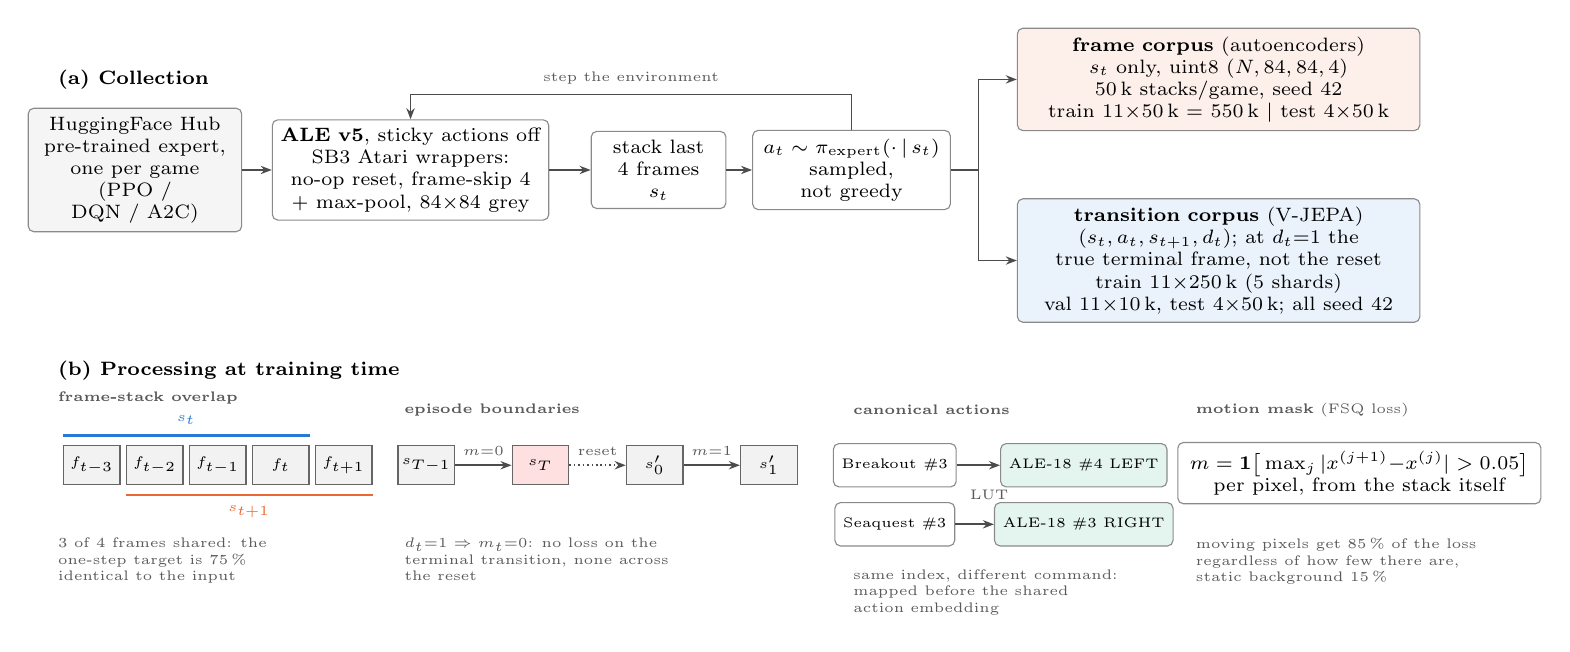
\begin{tikzpicture}[
  font=\scriptsize,
  box/.style={draw=cGray, rounded corners=2pt, align=center, inner sep=3pt, fill=white, minimum height=0.9cm},
  arr/.style={-{Stealth[length=4pt]}, draw=black!70, line width=0.6pt},
  fr/.style={draw=black!60, minimum width=0.72cm, minimum height=0.5cm, inner sep=0pt, font=\tiny},
  lab/.style={font=\tiny, text=black!65},
  ttl/.style={font=\scriptsize\bfseries, anchor=west}]

  % =========================================================== (a) collection
  \node[ttl] at (-1.1,3.35) {(a) Collection};
  \node[box, fill=gray!8, text width=2.5cm] (hub) at (0,2.2)
    {HuggingFace Hub\\pre-trained expert,\\one per game\\(PPO / DQN / A2C)};
  \node[box, text width=3.3cm] (env) at (3.5,2.2)
    {\textbf{ALE v5}, sticky actions off\\SB3 Atari wrappers: no-op reset, frame-skip 4 + max-pool, $84{\times}84$ grey};
  \node[box, text width=1.5cm] (stk) at (6.65,2.2) {stack last\\4 frames\\$s_t$};
  \node[box, text width=2.3cm] (pol) at (9.1,2.2) {$a_t\sim\pi_{\text{expert}}(\cdot\,|\,s_t)$\\sampled, not greedy};
  \draw[arr] (hub) -- (env); \draw[arr] (env) -- (stk); \draw[arr] (stk) -- (pol);
  \draw[arr] (pol.north) -- ++(0,0.45) -| node[pos=0.25, above, lab]{step the environment} (env.north);

  \node[box, fill=cFsqF!10, text width=4.9cm, anchor=west] (c1) at (11.2,3.35)
    {\textbf{frame corpus} (autoencoders)\\$s_t$ only, uint8 $(N,84,84,4)$\\50\,k stacks/game, seed 42\\train 11${\times}$50\,k = 550\,k $\mid$ test 4${\times}$50\,k};
  \node[box, fill=cNat!10, text width=4.9cm, anchor=west] (c2) at (11.2,1.05)
    {\textbf{transition corpus} (V-JEPA)\\$(s_t,a_t,s_{t+1},d_t)$; at $d_t{=}1$ the\\true terminal frame, not the reset\\train 11${\times}$250\,k (5 shards)\\val 11${\times}$10\,k, test 4${\times}$50\,k; all seed 42};
  \draw[arr] (pol.east) -- ++(0.35,0) |- (c1.west);
  \draw[arr] (pol.east) -- ++(0.35,0) |- (c2.west);

  % =========================================================== (b) processing
  \node[ttl] at (-1.1,-0.35) {(b) Processing at training time};

  % --- b1 frame overlap
  \node[lab, anchor=west] at (-1.1,-0.7) {\textbf{frame-stack overlap}};
  \foreach \i/\t in {0/$f_{t-3}$,1/$f_{t-2}$,2/$f_{t-1}$,3/$f_{t}$,4/$f_{t+1}$}
    {\node[fr, fill=gray!10] (f\i) at (-0.55+\i*0.8,-1.55) {\t};}
  \draw[cNat, line width=1pt] ([yshift=0.12cm]f0.north west) -- ([yshift=0.12cm]f3.north east)
     node[midway, above, font=\tiny, text=cNat] {$s_t$};
  \draw[cFsqF, line width=1pt] ([yshift=-0.12cm]f1.south west) -- ([yshift=-0.12cm]f4.south east)
     node[midway, below, font=\tiny, text=cFsqF] {$s_{t+1}$};
  \node[lab, align=left, anchor=north west] at (-1.1,-2.35) {3 of 4 frames shared: the\\one-step target is 75\,\%\\identical to the input};

  % --- b2 terminal mask
  \node[lab, anchor=west] at (3.3,-0.85) {\textbf{episode boundaries}};
  \node[fr, fill=gray!10] (e1) at (3.7,-1.55) {$s_{T-1}$};
  \node[fr, fill=red!12] (e2) at (5.15,-1.55) {$s_T$};
  \node[fr, fill=gray!10] (e3) at (6.6,-1.55) {$s'_0$};
  \node[fr, fill=gray!10] (e4) at (8.05,-1.55) {$s'_1$};
  \draw[arr] (e1) -- node[above, lab]{$m{=}0$} (e2);
  \draw[arr, densely dotted] (e2) -- node[above, lab]{reset} (e3);
  \draw[arr] (e3) -- node[above, lab]{$m{=}1$} (e4);
  \node[lab, align=left, anchor=north west] at (3.3,-2.35) {$d_t{=}1\Rightarrow m_t{=}0$: no loss on the\\terminal transition, none across\\the reset};

  % --- b3 action canonicalisation
  \node[lab, anchor=west] at (9.0,-0.85) {\textbf{canonical actions}};
  \node[box, minimum height=0.55cm, font=\tiny] (bk) at (9.65,-1.55) {Breakout \#3};
  \node[box, minimum height=0.55cm, font=\tiny] (sq) at (9.65,-2.3) {Seaquest \#3};
  \node[box, minimum height=0.55cm, font=\tiny, fill=cFsqJ!12] (l4) at (12.05,-1.55) {ALE-18 \#4 LEFT};
  \node[box, minimum height=0.55cm, font=\tiny, fill=cFsqJ!12] (r3) at (12.05,-2.3) {ALE-18 \#3 RIGHT};
  \draw[arr] (bk) -- (l4); \node[lab] at (10.85,-1.93) {LUT}; \draw[arr] (sq) -- (r3);
  \node[lab, align=left, anchor=north west] at (9.0,-2.75) {same index, different command:\\mapped before the shared\\action embedding};

  % --- b4 motion mask
  \node[lab, anchor=west] at (13.35,-0.85) {\textbf{motion mask} (FSQ loss)};
  \node[box, minimum height=0.55cm, text width=4.4cm, font=\scriptsize] (mm) at (15.55,-1.65)
    {\mbox{$m=\mathbf{1}\big[\max_j|x^{(j+1)}{-}x^{(j)}|>0.05\big]$}\\per pixel, from the stack itself};
  \node[lab, align=left, anchor=north west] at (13.35,-2.35) {moving pixels get 85\,\% of the loss\\regardless of how few there are,\\static background 15\,\%};
\end{tikzpicture}}

\resizebox{\textwidth}{!}{%
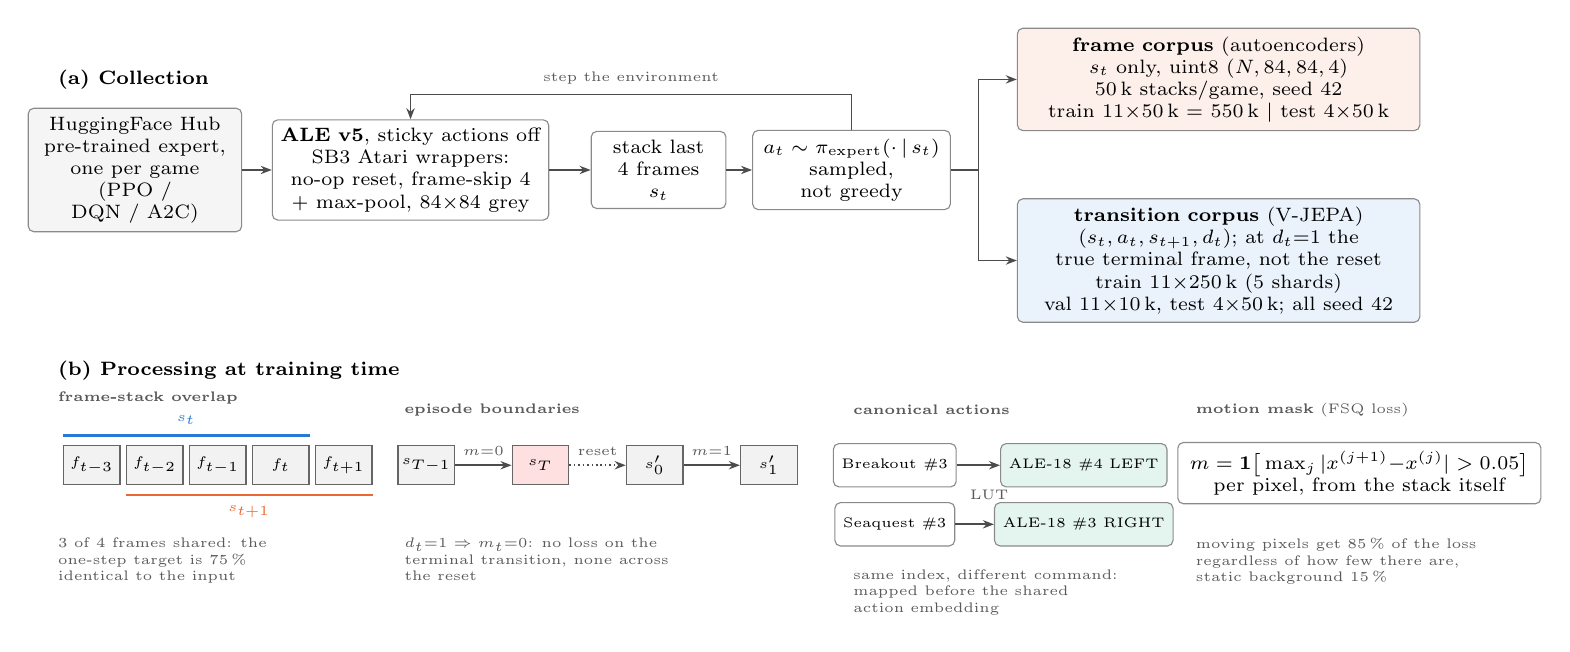
\begin{tikzpicture}[
  font=\scriptsize,
  box/.style={draw=cGray, rounded corners=2pt, align=center, inner sep=3pt, fill=white, minimum height=0.9cm},
  arr/.style={-{Stealth[length=4pt]}, draw=black!70, line width=0.6pt},
  fr/.style={draw=black!60, minimum width=0.72cm, minimum height=0.5cm, inner sep=0pt, font=\tiny},
  lab/.style={font=\tiny, text=black!65},
  ttl/.style={font=\scriptsize\bfseries, anchor=west}]

  % =========================================================== (a) collection
  \node[ttl] at (-1.1,3.35) {(a) Collection};
  \node[box, fill=gray!8, text width=2.5cm] (hub) at (0,2.2)
    {HuggingFace Hub\\pre-trained expert,\\one per game\\(PPO / DQN / A2C)};
  \node[box, text width=3.3cm] (env) at (3.5,2.2)
    {\textbf{ALE v5}, sticky actions off\\SB3 Atari wrappers: no-op reset, frame-skip 4 + max-pool, $84{\times}84$ grey};
  \node[box, text width=1.5cm] (stk) at (6.65,2.2) {stack last\\4 frames\\$s_t$};
  \node[box, text width=2.3cm] (pol) at (9.1,2.2) {$a_t\sim\pi_{\text{expert}}(\cdot\,|\,s_t)$\\sampled, not greedy};
  \draw[arr] (hub) -- (env); \draw[arr] (env) -- (stk); \draw[arr] (stk) -- (pol);
  \draw[arr] (pol.north) -- ++(0,0.45) -| node[pos=0.25, above, lab]{step the environment} (env.north);

  \node[box, fill=cFsqF!10, text width=4.9cm, anchor=west] (c1) at (11.2,3.35)
    {\textbf{frame corpus} (autoencoders)\\$s_t$ only, uint8 $(N,84,84,4)$\\50\,k stacks/game, seed 42\\train 11${\times}$50\,k = 550\,k $\mid$ test 4${\times}$50\,k};
  \node[box, fill=cNat!10, text width=4.9cm, anchor=west] (c2) at (11.2,1.05)
    {\textbf{transition corpus} (V-JEPA)\\$(s_t,a_t,s_{t+1},d_t)$; at $d_t{=}1$ the\\true terminal frame, not the reset\\train 11${\times}$250\,k (5 shards)\\val 11${\times}$10\,k, test 4${\times}$50\,k; all seed 42};
  \draw[arr] (pol.east) -- ++(0.35,0) |- (c1.west);
  \draw[arr] (pol.east) -- ++(0.35,0) |- (c2.west);

  % =========================================================== (b) processing
  \node[ttl] at (-1.1,-0.35) {(b) Processing at training time};

  % --- b1 frame overlap
  \node[lab, anchor=west] at (-1.1,-0.7) {\textbf{frame-stack overlap}};
  \foreach \i/\t in {0/$f_{t-3}$,1/$f_{t-2}$,2/$f_{t-1}$,3/$f_{t}$,4/$f_{t+1}$}
    {\node[fr, fill=gray!10] (f\i) at (-0.55+\i*0.8,-1.55) {\t};}
  \draw[cNat, line width=1pt] ([yshift=0.12cm]f0.north west) -- ([yshift=0.12cm]f3.north east)
     node[midway, above, font=\tiny, text=cNat] {$s_t$};
  \draw[cFsqF, line width=1pt] ([yshift=-0.12cm]f1.south west) -- ([yshift=-0.12cm]f4.south east)
     node[midway, below, font=\tiny, text=cFsqF] {$s_{t+1}$};
  \node[lab, align=left, anchor=north west] at (-1.1,-2.35) {3 of 4 frames shared: the\\one-step target is 75\,\%\\identical to the input};

  % --- b2 terminal mask
  \node[lab, anchor=west] at (3.3,-0.85) {\textbf{episode boundaries}};
  \node[fr, fill=gray!10] (e1) at (3.7,-1.55) {$s_{T-1}$};
  \node[fr, fill=red!12] (e2) at (5.15,-1.55) {$s_T$};
  \node[fr, fill=gray!10] (e3) at (6.6,-1.55) {$s'_0$};
  \node[fr, fill=gray!10] (e4) at (8.05,-1.55) {$s'_1$};
  \draw[arr] (e1) -- node[above, lab]{$m{=}0$} (e2);
  \draw[arr, densely dotted] (e2) -- node[above, lab]{reset} (e3);
  \draw[arr] (e3) -- node[above, lab]{$m{=}1$} (e4);
  \node[lab, align=left, anchor=north west] at (3.3,-2.35) {$d_t{=}1\Rightarrow m_t{=}0$: no loss on the\\terminal transition, none across\\the reset};

  % --- b3 action canonicalisation
  \node[lab, anchor=west] at (9.0,-0.85) {\textbf{canonical actions}};
  \node[box, minimum height=0.55cm, font=\tiny] (bk) at (9.65,-1.55) {Breakout \#3};
  \node[box, minimum height=0.55cm, font=\tiny] (sq) at (9.65,-2.3) {Seaquest \#3};
  \node[box, minimum height=0.55cm, font=\tiny, fill=cFsqJ!12] (l4) at (12.05,-1.55) {ALE-18 \#4 LEFT};
  \node[box, minimum height=0.55cm, font=\tiny, fill=cFsqJ!12] (r3) at (12.05,-2.3) {ALE-18 \#3 RIGHT};
  \draw[arr] (bk) -- (l4); \node[lab] at (10.85,-1.93) {LUT}; \draw[arr] (sq) -- (r3);
  \node[lab, align=left, anchor=north west] at (9.0,-2.75) {same index, different command:\\mapped before the shared\\action embedding};

  % --- b4 motion mask
  \node[lab, anchor=west] at (13.35,-0.85) {\textbf{motion mask} (FSQ loss)};
  \node[box, minimum height=0.55cm, text width=4.4cm, font=\scriptsize] (mm) at (15.55,-1.65)
    {\mbox{$m=\mathbf{1}\big[\max_j|x^{(j+1)}{-}x^{(j)}|>0.05\big]$}\\per pixel, from the stack itself};
  \node[lab, align=left, anchor=north west] at (13.35,-2.35) {moving pixels get 85\,\% of the loss\\regardless of how few there are,\\static background 15\,\%};
\end{tikzpicture}}

\resizebox{\textwidth}{!}{%
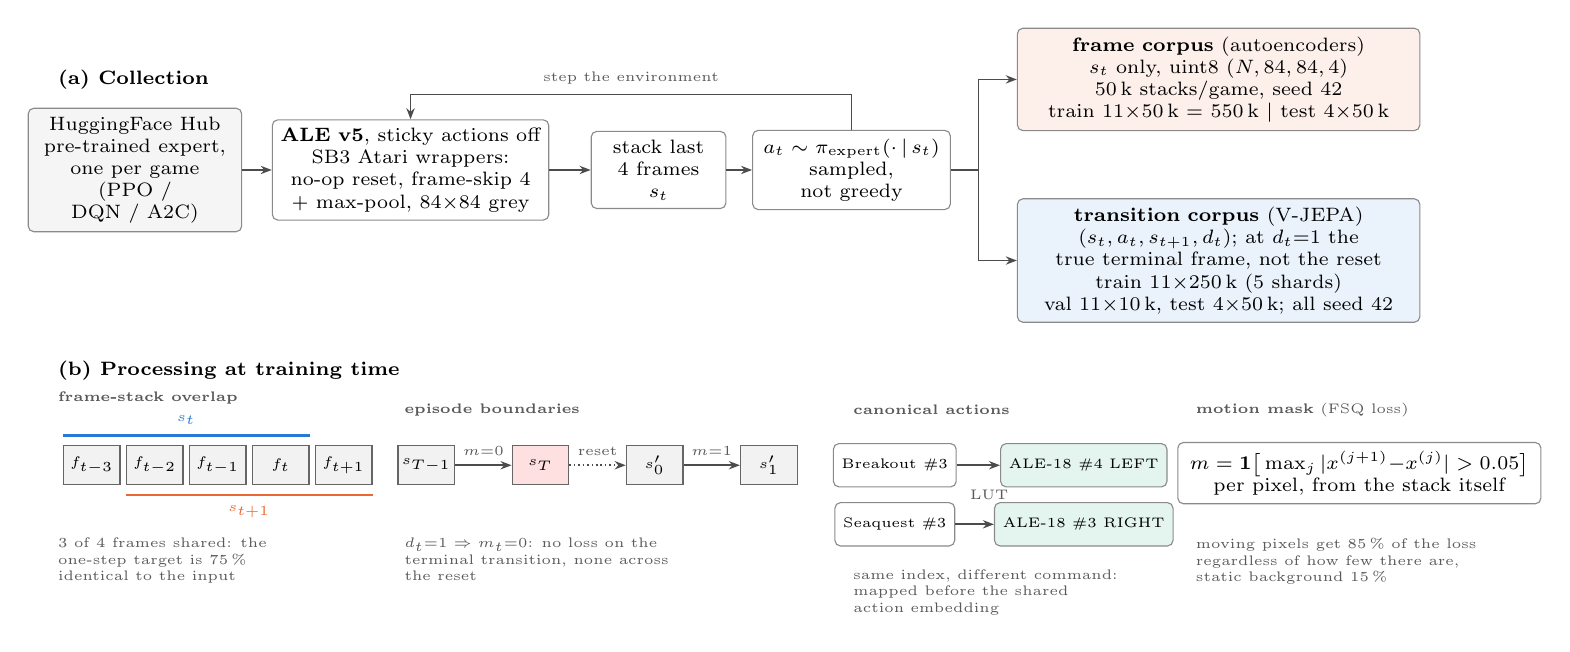
\begin{tikzpicture}[
  font=\scriptsize,
  box/.style={draw=cGray, rounded corners=2pt, align=center, inner sep=3pt, fill=white, minimum height=0.9cm},
  arr/.style={-{Stealth[length=4pt]}, draw=black!70, line width=0.6pt},
  fr/.style={draw=black!60, minimum width=0.72cm, minimum height=0.5cm, inner sep=0pt, font=\tiny},
  lab/.style={font=\tiny, text=black!65},
  ttl/.style={font=\scriptsize\bfseries, anchor=west}]

  % =========================================================== (a) collection
  \node[ttl] at (-1.1,3.35) {(a) Collection};
  \node[box, fill=gray!8, text width=2.5cm] (hub) at (0,2.2)
    {HuggingFace Hub\\pre-trained expert,\\one per game\\(PPO / DQN / A2C)};
  \node[box, text width=3.3cm] (env) at (3.5,2.2)
    {\textbf{ALE v5}, sticky actions off\\SB3 Atari wrappers: no-op reset, frame-skip 4 + max-pool, $84{\times}84$ grey};
  \node[box, text width=1.5cm] (stk) at (6.65,2.2) {stack last\\4 frames\\$s_t$};
  \node[box, text width=2.3cm] (pol) at (9.1,2.2) {$a_t\sim\pi_{\text{expert}}(\cdot\,|\,s_t)$\\sampled, not greedy};
  \draw[arr] (hub) -- (env); \draw[arr] (env) -- (stk); \draw[arr] (stk) -- (pol);
  \draw[arr] (pol.north) -- ++(0,0.45) -| node[pos=0.25, above, lab]{step the environment} (env.north);

  \node[box, fill=cFsqF!10, text width=4.9cm, anchor=west] (c1) at (11.2,3.35)
    {\textbf{frame corpus} (autoencoders)\\$s_t$ only, uint8 $(N,84,84,4)$\\50\,k stacks/game, seed 42\\train 11${\times}$50\,k = 550\,k $\mid$ test 4${\times}$50\,k};
  \node[box, fill=cNat!10, text width=4.9cm, anchor=west] (c2) at (11.2,1.05)
    {\textbf{transition corpus} (V-JEPA)\\$(s_t,a_t,s_{t+1},d_t)$; at $d_t{=}1$ the\\true terminal frame, not the reset\\train 11${\times}$250\,k (5 shards)\\val 11${\times}$10\,k, test 4${\times}$50\,k; all seed 42};
  \draw[arr] (pol.east) -- ++(0.35,0) |- (c1.west);
  \draw[arr] (pol.east) -- ++(0.35,0) |- (c2.west);

  % =========================================================== (b) processing
  \node[ttl] at (-1.1,-0.35) {(b) Processing at training time};

  % --- b1 frame overlap
  \node[lab, anchor=west] at (-1.1,-0.7) {\textbf{frame-stack overlap}};
  \foreach \i/\t in {0/$f_{t-3}$,1/$f_{t-2}$,2/$f_{t-1}$,3/$f_{t}$,4/$f_{t+1}$}
    {\node[fr, fill=gray!10] (f\i) at (-0.55+\i*0.8,-1.55) {\t};}
  \draw[cNat, line width=1pt] ([yshift=0.12cm]f0.north west) -- ([yshift=0.12cm]f3.north east)
     node[midway, above, font=\tiny, text=cNat] {$s_t$};
  \draw[cFsqF, line width=1pt] ([yshift=-0.12cm]f1.south west) -- ([yshift=-0.12cm]f4.south east)
     node[midway, below, font=\tiny, text=cFsqF] {$s_{t+1}$};
  \node[lab, align=left, anchor=north west] at (-1.1,-2.35) {3 of 4 frames shared: the\\one-step target is 75\,\%\\identical to the input};

  % --- b2 terminal mask
  \node[lab, anchor=west] at (3.3,-0.85) {\textbf{episode boundaries}};
  \node[fr, fill=gray!10] (e1) at (3.7,-1.55) {$s_{T-1}$};
  \node[fr, fill=red!12] (e2) at (5.15,-1.55) {$s_T$};
  \node[fr, fill=gray!10] (e3) at (6.6,-1.55) {$s'_0$};
  \node[fr, fill=gray!10] (e4) at (8.05,-1.55) {$s'_1$};
  \draw[arr] (e1) -- node[above, lab]{$m{=}0$} (e2);
  \draw[arr, densely dotted] (e2) -- node[above, lab]{reset} (e3);
  \draw[arr] (e3) -- node[above, lab]{$m{=}1$} (e4);
  \node[lab, align=left, anchor=north west] at (3.3,-2.35) {$d_t{=}1\Rightarrow m_t{=}0$: no loss on the\\terminal transition, none across\\the reset};

  % --- b3 action canonicalisation
  \node[lab, anchor=west] at (9.0,-0.85) {\textbf{canonical actions}};
  \node[box, minimum height=0.55cm, font=\tiny] (bk) at (9.65,-1.55) {Breakout \#3};
  \node[box, minimum height=0.55cm, font=\tiny] (sq) at (9.65,-2.3) {Seaquest \#3};
  \node[box, minimum height=0.55cm, font=\tiny, fill=cFsqJ!12] (l4) at (12.05,-1.55) {ALE-18 \#4 LEFT};
  \node[box, minimum height=0.55cm, font=\tiny, fill=cFsqJ!12] (r3) at (12.05,-2.3) {ALE-18 \#3 RIGHT};
  \draw[arr] (bk) -- (l4); \node[lab] at (10.85,-1.93) {LUT}; \draw[arr] (sq) -- (r3);
  \node[lab, align=left, anchor=north west] at (9.0,-2.75) {same index, different command:\\mapped before the shared\\action embedding};

  % --- b4 motion mask
  \node[lab, anchor=west] at (13.35,-0.85) {\textbf{motion mask} (FSQ loss)};
  \node[box, minimum height=0.55cm, text width=4.4cm, font=\scriptsize] (mm) at (15.55,-1.65)
    {\mbox{$m=\mathbf{1}\big[\max_j|x^{(j+1)}{-}x^{(j)}|>0.05\big]$}\\per pixel, from the stack itself};
  \node[lab, align=left, anchor=north west] at (13.35,-2.35) {moving pixels get 85\,\% of the loss\\regardless of how few there are,\\static background 15\,\%};
\end{tikzpicture}}

\caption{(a)~Data collection with pre-trained expert agents and the two resulting corpora.
(b)~Processing at training time: frame-stack overlap, masking of episode-ending
transitions, mapping of game-specific action indices to the canonical ALE-18 set, and the
motion mask of the FSQ-VAE loss.}
\label{fig:data}
\end{figure}

% =========================================================================
\section{The Games}
\label{sec:games}

\Cref{fig:games} shows all 15 games as the encoder sees them. Eleven are used for pre-training
and four are held out to test generalisation. Every game produces a tensor of the same shape,
but the content varies considerably (\cref{tab:games}), and a shared encoder has to
cope with all of these differences at once.

\begin{figure}[!htbp]
\centering
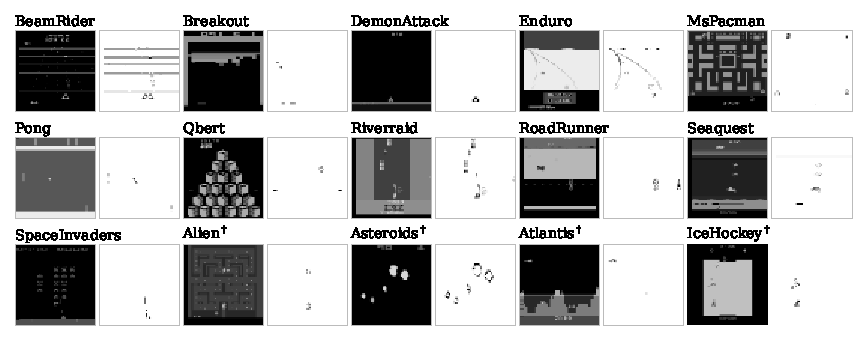
\includegraphics[width=\textwidth]{figures/games_grid.pdf}
\caption{All 15 games as the encoder sees them: the newest frame $t$ of an expert frame stack
(left of each pair) and $|x_{t+1}-x_t|$, the change to the next frame (right, inverted, per-image
contrast). $^\dagger$\,held-out games. Frames from the data specimen sheet of the transition
corpus.}
\label{fig:games}
\end{figure}

\begin{table}[!htbp]
\centering
\caption{How the games differ. $|\mathcal{A}|$: minimal action set; pixel mean (0--255) and
black \% of the frames; moving \%: pixels that change within a stack ($\delta=0.05$); steps per
terminal (the Atari wrappers also end an episode on a life loss); top action: share of the
expert's most frequent action. Computed on 50\,k transitions per game of the transition
corpus; $^\dagger$\,held-out.}
\label{tab:games}
\scriptsize\setlength{\tabcolsep}{2.2pt}
\begin{tabular}{@{}llccrrrrr@{}}
\toprule
Game & Type & $|\mathcal{A}|$ & Expert & Pix. & Black & Mov. & Steps/ & Top \\
 & & & & mean & \% & \% & term. & act.\ \% \\
\midrule
\tabinput{tables/games_rows.tex}
\bottomrule
\end{tabular}
\end{table}

\paragraph{Appearance.} The mean brightness ranges from 5 (DemonAttack) to 105 (Pong), and
the share of black pixels from 1\% (Pong) to 95\% (Asteroids). Shooters on a black background
(BeamRider, DemonAttack, SpaceInvaders, Asteroids) are 79--95\% black, whereas Pong, Riverraid,
Seaquest and the maze games fill most of the screen (1--20\% black).

\paragraph{Motion.} In most games, fewer than 4\% of the pixels change within a frame stack
(Pong 1.7\%, Breakout 1.4\%, IceHockey 1.1\%). Only BeamRider (34\%) and Riverraid (10\%) move
large parts of the screen; the other scrolling and pseudo-3D games (RoadRunner 7.4\%, Enduro
6.9\%) change about as much as Asteroids and Atlantis (6\%). The objects relevant for playing are thus usually a few small sprites on a static background,
which a loss that weights all pixels equally can almost ignore.

\paragraph{Actions and episode length.} The number of actions ranges from 4 to 18, and the same
action index means a different joystick command in different games, so a shared action
embedding requires a common action set (\cref{sec:models}). Episodes last from about
120 steps (Atlantis) to 12\,500 steps (Enduro). The expert data is also unevenly varied: the most frequent expert action covers 8\% of the
steps in Seaquest, but 67\% in RoadRunner and 99\% in Asteroids, so for such games the data
rarely shows the effect of a different action.

% =========================================================================
\section{Models}
\label{sec:models}

All encoders receive the same input $x\in[0,1]^{4\times84\times84}$. After pre-training, only the encoder is kept, and its output is passed to the actor and critic
of PPO. The baseline is a NatureCNN with a 512-dimensional feature, trained
from scratch.

\FloatBarrier
\subsection{Autoencoders}

I first trained a Gaussian VAE~\cite{kingma2014vae} with the NatureCNN layers as encoder and
a 256-dimensional latent vector (\cref{tab:pretrain}). Its encoder reduces the frame to a
$7\times7$ feature map before the bottleneck, so each cell is responsible for a $12\times12$
pixel region, much larger than a ball or a bullet. I therefore also trained spatial, discrete
bottlenecks.

\paragraph{Residual VQ-VAE.} This model keeps a finer $21\times21$ latent grid, using two
stride-2 convolutions and two residual blocks. Each 64-dimensional latent cell is replaced by
the closest of $K=512$ codebook vectors. Since this rounding step has no gradient, the
gradient is simply copied from the decoder input to the encoder output (the straight-through
trick). The codebook is updated with exponential moving averages
($\gamma=0.99$), the commitment weight is $\beta=0.25$, and codes that are no longer used are
re-initialised. Inspecting the reconstructions showed that small moving objects were often
missing. To address this, I trained a second version in which the error on moving pixels,
$m=\mathbf{1}[\max_j|x^{(j+1)}-x^{(j)}|>0.05]$, is weighted ten times higher.

\paragraph{FSQ-VAE.} Finite Scalar Quantisation~\cite{mentzer2024fsq} removes the codebook
entirely. A three-layer convolutional encoder outputs four channels, and each channel is
rounded to a fixed number of levels, $L=[8,5,5,3]$, giving 600 possible values per latent cell.
There is no codebook, no commitment loss and no unused codes. My first version
used transposed convolutions in the decoder, which caused checkerboard artefacts on the flat
Atari backgrounds, so I replaced them with upsampling followed by standard convolutions.
Instead of a fixed factor of ten, the final loss normalises moving and static pixels
separately:
\begin{equation}
  \mathcal{L}_{\text{bal}} = w\,\tfrac{\sum m\odot(\hat x-x)^2}{\sum m}
  +(1-w)\,\tfrac{\sum (1-m)\odot(\hat x-x)^2}{\sum (1-m)},\qquad w=0.85.
\end{equation}
Moving pixels thus always account for 85\% of the loss, however few of them there are.
For PPO, the feature is the flattened $4\times21\times21$ quantised grid (1\,764 values).

\FloatBarrier
\subsection{Action- and Game-Conditioned V-JEPA}

A JEPA does not reconstruct pixels. Instead, it learns to predict the \emph{representation}
of the next observation~\cite{lecun2022path}. If the predictor is also given the action, the
model becomes a latent world model, similar to SPR~\cite{schwarzer2021spr}. The name follows
V-JEPA~\cite{bardes2024vjepa}, which learns from video by predicting the representations of
masked regions; my model instead predicts the whole next frame stack. \Cref{fig:jepa}
shows the final model. A $14\times14$ patch embedding turns a frame stack into 36 tokens of
size 256. The context encoder $E_\theta$, a six-layer transformer, encodes $s_t$, and the
target encoder $\bar E$, an exponential moving average (EMA) of $E_\theta$ with $\tau=0.996$
that receives no gradients~\cite{assran2023ijepa}, encodes $s_{t+1}$. A three-layer predictor
$P_\psi$ gets the context tokens together with an action token and a game token, and has to
predict the target tokens:
\begin{equation}
  \mathcal{L}_{\text{JEPA}}=\frac{\sum_i m_i\,\big\|P_\psi\big(E_\theta(s_t^i,e^i),a_t^i,e^i\big)
  -\operatorname{sg}\big(\bar E(s_{t+1}^i,e^i)\big)\big\|_2^2}{\sum_i m_i},
\end{equation}
where $m_i=0$ for transitions that end an episode.

\begin{figure}[!htbp]
\centering
% V-JEPA v2 architecture (atari-DQN-v2/JEPA.py), used as % V-JEPA v2 architecture (atari-DQN-v2/JEPA.py), used as % V-JEPA v2 architecture (atari-DQN-v2/JEPA.py), used as \input{figures/jepa_arch}
\resizebox{\textwidth}{!}{%
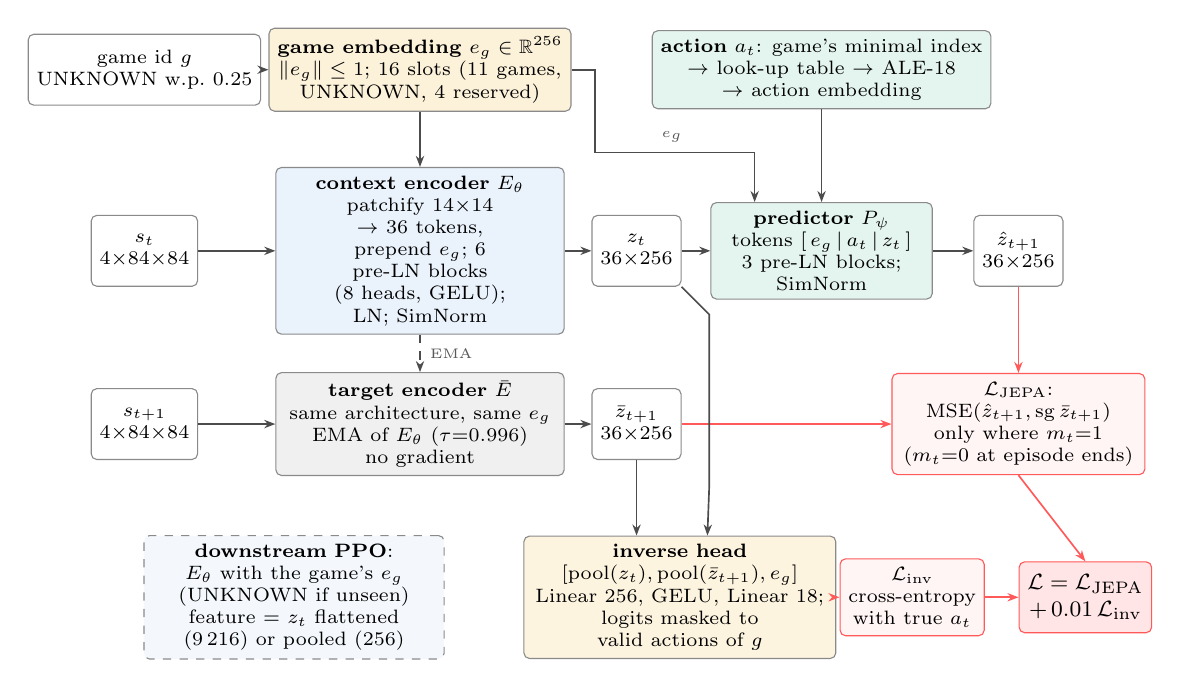
\begin{tikzpicture}[
  font=\scriptsize,
  box/.style={draw=cGray, rounded corners=2pt, align=center, inner sep=3pt, fill=white,
              minimum height=0.9cm},
  arr/.style={-{Stealth[length=4pt]}, draw=black!70, line width=0.6pt},
  larr/.style={-{Stealth[length=4pt]}, draw=red!65, line width=0.6pt},
  lab/.style={font=\tiny, text=black!65}]

  % ---------------------------------------------------------------- conditioning (top row)
  \node[box] (drop) at (0,4.5) {game id $g$\\UNKNOWN w.p.\ 0.25};
  \node[box, fill=cJep!15] (env) at (3.5,4.5)
    {\textbf{game embedding} $e_g\in\mathbb{R}^{256}$\\$\|e_g\|\le1$; 16 slots (11 games,\\UNKNOWN, 4 reserved)};
  \node[box, fill=cFsqJ!12] (act) at (8.6,4.5)
    {\textbf{action} $a_t$: game's minimal index\\$\to$ look-up table $\to$ ALE-18\\$\to$ action embedding};
  \draw[arr] (drop) -- (env);

  % ---------------------------------------------------------------- online branch
  \node[box] (st) at (0,2.2) {$s_t$\\$4{\times}84{\times}84$};
  \node[box, fill=cNat!10, text width=3.45cm] (ce) at (3.5,2.2)
    {\textbf{context encoder} $E_\theta$\\patchify $14{\times}14$ $\to$ 36 tokens,\\prepend $e_g$; 6 pre-LN blocks\\(8 heads, GELU); LN; SimNorm};
  \node[box] (zt) at (6.25,2.2) {$z_t$\\$36{\times}256$};
  \node[box, fill=cFsqJ!12, text width=2.6cm] (pr) at (8.6,2.2)
    {\textbf{predictor} $P_\psi$\\tokens $[\,e_g\,|\,a_t\,|\,z_t\,]$\\3 pre-LN blocks; SimNorm};
  \node[box] (zh) at (11.1,2.2) {$\hat z_{t+1}$\\$36{\times}256$};
  \draw[arr] (st) -- (ce); \draw[arr] (ce) -- (zt); \draw[arr] (zt) -- (pr); \draw[arr] (pr) -- (zh);
  \draw[arr] (env) -- (ce);
  \draw[arr] (act) -- (pr);
  \coordinate (ebend) at (7.75,3.45);
  \draw[arr] (env.east) -- ++(0.3,0) |- (ebend) -- (ebend |- pr.north);
  \node[lab, above] at (6.7,3.45) {$e_g$};

  % ---------------------------------------------------------------- target branch
  \node[box] (sn) at (0,0) {$s_{t+1}$\\$4{\times}84{\times}84$};
  \node[box, fill=gray!12, text width=3.45cm] (te) at (3.5,0)
    {\textbf{target encoder} $\bar E$\\same architecture, same $e_g$\\EMA of $E_\theta$ ($\tau{=}0.996$)\\no gradient};
  \node[box] (zb) at (6.25,0) {$\bar z_{t+1}$\\$36{\times}256$};
  \draw[arr] (sn) -- (te); \draw[arr] (te) -- (zb);
  \draw[arr, dashed] (ce) -- node[right, lab]{EMA} (te);

  % ---------------------------------------------------------------- losses
  \node[box, draw=red!65, fill=red!4, text width=3.0cm] (lj) at (11.1,0)
    {$\mathcal{L}_{\text{JEPA}}$: MSE$(\hat z_{t+1},\operatorname{sg}\bar z_{t+1})$\\only where $m_t{=}1$\\($m_t{=}0$ at episode ends)};
  \draw[larr] (zh) -- (lj);
  \draw[larr] (zb) -- (lj);

  \node[box, fill=cJep!12, text width=3.75cm] (inv) at (6.8,-2.2)
    {\textbf{inverse head}\\$[\operatorname{pool}(z_t),\operatorname{pool}(\bar z_{t+1}),e_g]$\\Linear 256, GELU, Linear 18;\\logits masked to valid actions of $g$};
  \draw[arr] (zt.south east) -- ++(0.35,-0.35) -- ++(0,-2.2) -- ([xshift=0.35cm]inv.north);
  \draw[arr] (zb) -- (zb |- inv.north);
  \node[box, draw=red!65, fill=red!4] (li) at (9.75,-2.2) {$\mathcal{L}_{\text{inv}}$\\cross-entropy\\with true $a_t$};
  \draw[larr] (inv) -- (li);
  \node[box, draw=red!65, fill=red!10, font=\footnotesize] (tot) at (11.95,-2.2)
    {$\mathcal{L}=\mathcal{L}_{\text{JEPA}}$\\$+\,0.01\,\mathcal{L}_{\text{inv}}$};
  \draw[larr] (li) -- (tot);
  \draw[larr] (lj.south) -- (tot.north);

  % ---------------------------------------------------------------- use in PPO
  \node[box, dashed, fill=cNat!5, text width=3.6cm] (ppo) at (1.9,-2.2)
    {\textbf{downstream PPO}: $E_\theta$ with the game's $e_g$ (UNKNOWN if unseen)\\feature = $z_t$ flattened (9\,216) or pooled (256)};
\end{tikzpicture}}

\resizebox{\textwidth}{!}{%
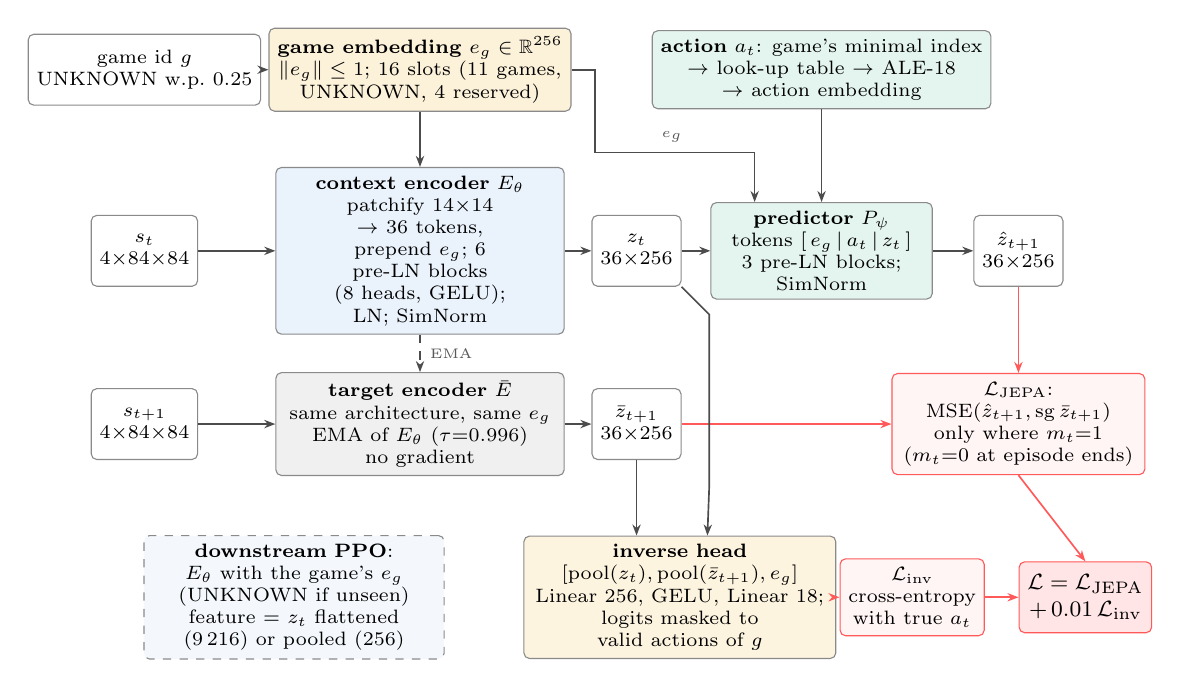
\begin{tikzpicture}[
  font=\scriptsize,
  box/.style={draw=cGray, rounded corners=2pt, align=center, inner sep=3pt, fill=white,
              minimum height=0.9cm},
  arr/.style={-{Stealth[length=4pt]}, draw=black!70, line width=0.6pt},
  larr/.style={-{Stealth[length=4pt]}, draw=red!65, line width=0.6pt},
  lab/.style={font=\tiny, text=black!65}]

  % ---------------------------------------------------------------- conditioning (top row)
  \node[box] (drop) at (0,4.5) {game id $g$\\UNKNOWN w.p.\ 0.25};
  \node[box, fill=cJep!15] (env) at (3.5,4.5)
    {\textbf{game embedding} $e_g\in\mathbb{R}^{256}$\\$\|e_g\|\le1$; 16 slots (11 games,\\UNKNOWN, 4 reserved)};
  \node[box, fill=cFsqJ!12] (act) at (8.6,4.5)
    {\textbf{action} $a_t$: game's minimal index\\$\to$ look-up table $\to$ ALE-18\\$\to$ action embedding};
  \draw[arr] (drop) -- (env);

  % ---------------------------------------------------------------- online branch
  \node[box] (st) at (0,2.2) {$s_t$\\$4{\times}84{\times}84$};
  \node[box, fill=cNat!10, text width=3.45cm] (ce) at (3.5,2.2)
    {\textbf{context encoder} $E_\theta$\\patchify $14{\times}14$ $\to$ 36 tokens,\\prepend $e_g$; 6 pre-LN blocks\\(8 heads, GELU); LN; SimNorm};
  \node[box] (zt) at (6.25,2.2) {$z_t$\\$36{\times}256$};
  \node[box, fill=cFsqJ!12, text width=2.6cm] (pr) at (8.6,2.2)
    {\textbf{predictor} $P_\psi$\\tokens $[\,e_g\,|\,a_t\,|\,z_t\,]$\\3 pre-LN blocks; SimNorm};
  \node[box] (zh) at (11.1,2.2) {$\hat z_{t+1}$\\$36{\times}256$};
  \draw[arr] (st) -- (ce); \draw[arr] (ce) -- (zt); \draw[arr] (zt) -- (pr); \draw[arr] (pr) -- (zh);
  \draw[arr] (env) -- (ce);
  \draw[arr] (act) -- (pr);
  \coordinate (ebend) at (7.75,3.45);
  \draw[arr] (env.east) -- ++(0.3,0) |- (ebend) -- (ebend |- pr.north);
  \node[lab, above] at (6.7,3.45) {$e_g$};

  % ---------------------------------------------------------------- target branch
  \node[box] (sn) at (0,0) {$s_{t+1}$\\$4{\times}84{\times}84$};
  \node[box, fill=gray!12, text width=3.45cm] (te) at (3.5,0)
    {\textbf{target encoder} $\bar E$\\same architecture, same $e_g$\\EMA of $E_\theta$ ($\tau{=}0.996$)\\no gradient};
  \node[box] (zb) at (6.25,0) {$\bar z_{t+1}$\\$36{\times}256$};
  \draw[arr] (sn) -- (te); \draw[arr] (te) -- (zb);
  \draw[arr, dashed] (ce) -- node[right, lab]{EMA} (te);

  % ---------------------------------------------------------------- losses
  \node[box, draw=red!65, fill=red!4, text width=3.0cm] (lj) at (11.1,0)
    {$\mathcal{L}_{\text{JEPA}}$: MSE$(\hat z_{t+1},\operatorname{sg}\bar z_{t+1})$\\only where $m_t{=}1$\\($m_t{=}0$ at episode ends)};
  \draw[larr] (zh) -- (lj);
  \draw[larr] (zb) -- (lj);

  \node[box, fill=cJep!12, text width=3.75cm] (inv) at (6.8,-2.2)
    {\textbf{inverse head}\\$[\operatorname{pool}(z_t),\operatorname{pool}(\bar z_{t+1}),e_g]$\\Linear 256, GELU, Linear 18;\\logits masked to valid actions of $g$};
  \draw[arr] (zt.south east) -- ++(0.35,-0.35) -- ++(0,-2.2) -- ([xshift=0.35cm]inv.north);
  \draw[arr] (zb) -- (zb |- inv.north);
  \node[box, draw=red!65, fill=red!4] (li) at (9.75,-2.2) {$\mathcal{L}_{\text{inv}}$\\cross-entropy\\with true $a_t$};
  \draw[larr] (inv) -- (li);
  \node[box, draw=red!65, fill=red!10, font=\footnotesize] (tot) at (11.95,-2.2)
    {$\mathcal{L}=\mathcal{L}_{\text{JEPA}}$\\$+\,0.01\,\mathcal{L}_{\text{inv}}$};
  \draw[larr] (li) -- (tot);
  \draw[larr] (lj.south) -- (tot.north);

  % ---------------------------------------------------------------- use in PPO
  \node[box, dashed, fill=cNat!5, text width=3.6cm] (ppo) at (1.9,-2.2)
    {\textbf{downstream PPO}: $E_\theta$ with the game's $e_g$ (UNKNOWN if unseen)\\feature = $z_t$ flattened (9\,216) or pooled (256)};
\end{tikzpicture}}

\resizebox{\textwidth}{!}{%
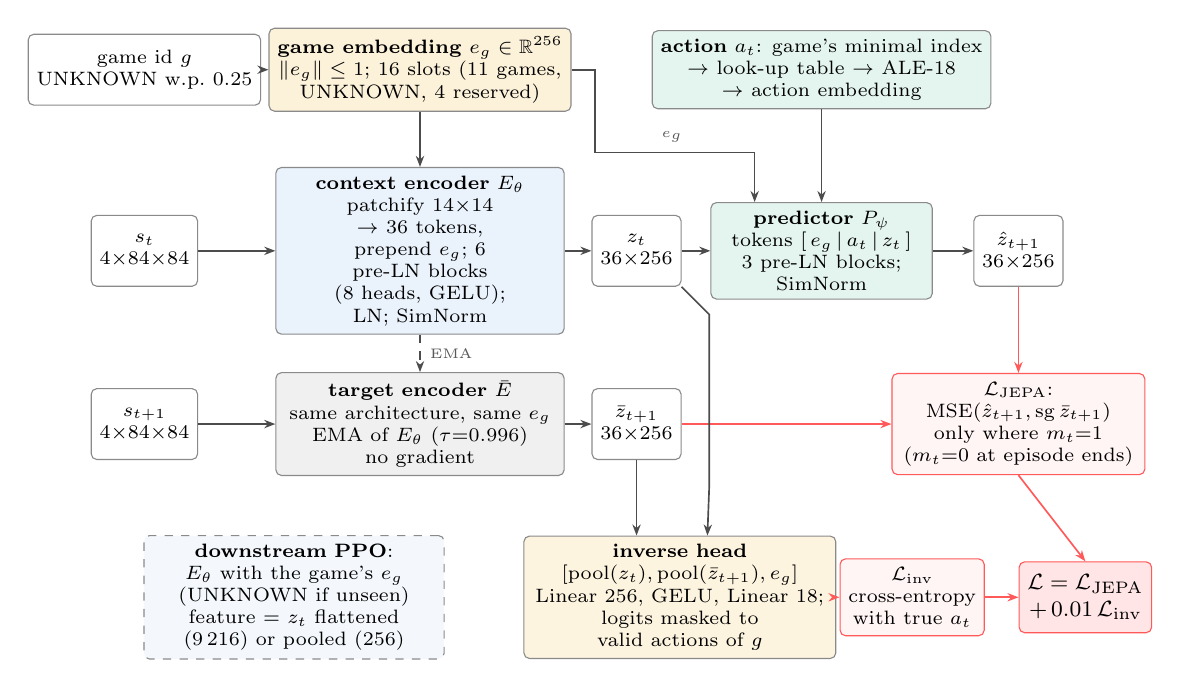
\begin{tikzpicture}[
  font=\scriptsize,
  box/.style={draw=cGray, rounded corners=2pt, align=center, inner sep=3pt, fill=white,
              minimum height=0.9cm},
  arr/.style={-{Stealth[length=4pt]}, draw=black!70, line width=0.6pt},
  larr/.style={-{Stealth[length=4pt]}, draw=red!65, line width=0.6pt},
  lab/.style={font=\tiny, text=black!65}]

  % ---------------------------------------------------------------- conditioning (top row)
  \node[box] (drop) at (0,4.5) {game id $g$\\UNKNOWN w.p.\ 0.25};
  \node[box, fill=cJep!15] (env) at (3.5,4.5)
    {\textbf{game embedding} $e_g\in\mathbb{R}^{256}$\\$\|e_g\|\le1$; 16 slots (11 games,\\UNKNOWN, 4 reserved)};
  \node[box, fill=cFsqJ!12] (act) at (8.6,4.5)
    {\textbf{action} $a_t$: game's minimal index\\$\to$ look-up table $\to$ ALE-18\\$\to$ action embedding};
  \draw[arr] (drop) -- (env);

  % ---------------------------------------------------------------- online branch
  \node[box] (st) at (0,2.2) {$s_t$\\$4{\times}84{\times}84$};
  \node[box, fill=cNat!10, text width=3.45cm] (ce) at (3.5,2.2)
    {\textbf{context encoder} $E_\theta$\\patchify $14{\times}14$ $\to$ 36 tokens,\\prepend $e_g$; 6 pre-LN blocks\\(8 heads, GELU); LN; SimNorm};
  \node[box] (zt) at (6.25,2.2) {$z_t$\\$36{\times}256$};
  \node[box, fill=cFsqJ!12, text width=2.6cm] (pr) at (8.6,2.2)
    {\textbf{predictor} $P_\psi$\\tokens $[\,e_g\,|\,a_t\,|\,z_t\,]$\\3 pre-LN blocks; SimNorm};
  \node[box] (zh) at (11.1,2.2) {$\hat z_{t+1}$\\$36{\times}256$};
  \draw[arr] (st) -- (ce); \draw[arr] (ce) -- (zt); \draw[arr] (zt) -- (pr); \draw[arr] (pr) -- (zh);
  \draw[arr] (env) -- (ce);
  \draw[arr] (act) -- (pr);
  \coordinate (ebend) at (7.75,3.45);
  \draw[arr] (env.east) -- ++(0.3,0) |- (ebend) -- (ebend |- pr.north);
  \node[lab, above] at (6.7,3.45) {$e_g$};

  % ---------------------------------------------------------------- target branch
  \node[box] (sn) at (0,0) {$s_{t+1}$\\$4{\times}84{\times}84$};
  \node[box, fill=gray!12, text width=3.45cm] (te) at (3.5,0)
    {\textbf{target encoder} $\bar E$\\same architecture, same $e_g$\\EMA of $E_\theta$ ($\tau{=}0.996$)\\no gradient};
  \node[box] (zb) at (6.25,0) {$\bar z_{t+1}$\\$36{\times}256$};
  \draw[arr] (sn) -- (te); \draw[arr] (te) -- (zb);
  \draw[arr, dashed] (ce) -- node[right, lab]{EMA} (te);

  % ---------------------------------------------------------------- losses
  \node[box, draw=red!65, fill=red!4, text width=3.0cm] (lj) at (11.1,0)
    {$\mathcal{L}_{\text{JEPA}}$: MSE$(\hat z_{t+1},\operatorname{sg}\bar z_{t+1})$\\only where $m_t{=}1$\\($m_t{=}0$ at episode ends)};
  \draw[larr] (zh) -- (lj);
  \draw[larr] (zb) -- (lj);

  \node[box, fill=cJep!12, text width=3.75cm] (inv) at (6.8,-2.2)
    {\textbf{inverse head}\\$[\operatorname{pool}(z_t),\operatorname{pool}(\bar z_{t+1}),e_g]$\\Linear 256, GELU, Linear 18;\\logits masked to valid actions of $g$};
  \draw[arr] (zt.south east) -- ++(0.35,-0.35) -- ++(0,-2.2) -- ([xshift=0.35cm]inv.north);
  \draw[arr] (zb) -- (zb |- inv.north);
  \node[box, draw=red!65, fill=red!4] (li) at (9.75,-2.2) {$\mathcal{L}_{\text{inv}}$\\cross-entropy\\with true $a_t$};
  \draw[larr] (inv) -- (li);
  \node[box, draw=red!65, fill=red!10, font=\footnotesize] (tot) at (11.95,-2.2)
    {$\mathcal{L}=\mathcal{L}_{\text{JEPA}}$\\$+\,0.01\,\mathcal{L}_{\text{inv}}$};
  \draw[larr] (li) -- (tot);
  \draw[larr] (lj.south) -- (tot.north);

  % ---------------------------------------------------------------- use in PPO
  \node[box, dashed, fill=cNat!5, text width=3.6cm] (ppo) at (1.9,-2.2)
    {\textbf{downstream PPO}: $E_\theta$ with the game's $e_g$ (UNKNOWN if unseen)\\feature = $z_t$ flattened (9\,216) or pooled (256)};
\end{tikzpicture}}

\caption{Action- and game-conditioned V-JEPA (v2), as implemented. The target
encoder is an EMA copy of the context encoder; only the context encoder is kept for PPO.}
\label{fig:jepa}
\end{figure}

My first version had a good loss curve, but a review showed that action indices meant
different commands in different games, the large dataset was loaded with the wrong axis order,
and the validation set contained only one game.
I therefore rebuilt the model (v2) following TD-MPC2~\cite{hansen2024tdmpc2}. First, all actions are mapped to the common set of 18 ALE actions. Second, each game
receives a learnable embedding $e_g$ with $\|e_g\|\le1$, which is added as a token to both
encoders and the predictor. With probability 0.25 it is replaced by a shared UNKNOWN
embedding, so that the model also learns a general ``Atari'' prior for unseen games. Third, all
latents are normalised with SimNorm, which splits them into 32 groups of $V=8$ values and
applies a softmax to each group. This keeps the latents bounded and makes collapse harder. Fourth,
an inverse-dynamics head~\cite{pathak2017icm} predicts the action $a_t$ from $z_t$,
$\bar z_{t+1}$ and $e_g$, only among the actions that are valid in the game. The total loss is
$\mathcal{L}=\mathcal{L}_{\text{JEPA}}+\lambda\mathcal{L}_{\text{inv}}$ with $\lambda=0.01$.

\paragraph{Training Step.} The target branch is computed without gradients, both losses are
averaged over the same unmasked samples, the gradients are clipped to a norm of 1.0, AdamW
updates the trainable parameters, and only then is the target encoder moved slightly towards the context encoder (\cref{tab:grad}). The target is thus a slowly moving goal that the context encoder cannot change directly,
which helps to prevent collapse to a constant output.
The inverse loss trains the encoder but \emph{not} the predictor, because its second input is
the target latent rather than the prediction.

\begin{table}[!htbp]
\centering
\caption{Gradient routing in the V-JEPA (12.48\,M parameters, 7.53\,M trainable).}
\label{tab:grad}
\footnotesize\setlength{\tabcolsep}{4pt}
\begin{tabular}{@{}lrccl@{}}
\toprule
Parameter group & Params & $\nabla\mathcal{L}_{\text{JEPA}}$ & $\nabla\mathcal{L}_{\text{inv}}$ & Update \\
\midrule
Context encoder (patchify, 6 blocks, LN) & 4.95\,M & yes & yes & AdamW \\
Predictor (action emb., 3 blocks, LN) & 2.37\,M & yes & no & AdamW \\
Inverse head ($768\to256\to18$) & 0.20\,M & no & yes & AdamW \\
Game embeddings ($16\times256$) & 0.004\,M & yes & yes & AdamW \\
Target encoder (copy of context enc.) & 4.95\,M & no & no & EMA only \\
\bottomrule
\end{tabular}
\end{table}

\paragraph{Using the Encoder in PPO.} The context encoder receives the game's own embedding (or UNKNOWN for
unseen games) and outputs $36\times256$ tokens, which are flattened into a 9\,216-dimensional
feature in the main runs and averaged into a 256-dimensional feature in a second set.

% =========================================================================
\section{Methodology}
\label{sec:method}


\Cref{tab:pretrain} lists the training setup of each encoder next to the setting of the paper
it is based on. The architectures follow the references, and most differences are due to scale: the JEPA
papers train large vision transformers on very large datasets, whereas my model has
12.5\,M parameters and was trained on a single GPU, so I used a smaller batch, a lower learning
rate, less weight decay and a fixed EMA momentum. For the V-JEPA, I kept the checkpoint with
the lowest total validation loss $\mathcal{L}_{\text{JEPA}}+\lambda\mathcal{L}_{\text{inv}}$
(epoch 90 of 92). This total fell during training because the inverse term improved, even though
the JEPA term alone rose after the first epochs (\cref{sec:pretrain-res}), so the selected
checkpoint lies well past the early, near-collapsed phase. A small sweep over
$\lambda\in\{0.003,0.01,0.03,0.1\}$ confirmed $\lambda=0.01$.

All PPO agents use the standard RL-Zoo Atari settings (last column of \cref{tab:pretrain},
with $\gamma=0.99$, $\lambda_{\text{GAE}}=0.95$, clip range 0.1 and entropy coefficient 0.01)
and the same 512-unit actor and critic heads. All agents were trained using
Stable-Baselines3. Performance is the mean training return over the last 10\% of training (steps 9--10\,M). As
score ranges differ widely between games, I convert it to the human-normalised score
HNS$=(\text{score}-\text{random})/(\text{human}-\text{random})$ with the reference scores of
Badia et al.~\cite{badia2020agent57} and mainly report the median over games. All numbers
except the Std-VAE and Res-VQ scores and the NatureCNN and V-JEPA scores on the held-out games,
which I only recorded in rounded form, are computed from the complete logs in Weights \& Biases. Each configuration was run with only one
seed, so small differences should be interpreted with caution~\cite{agarwal2021precipice}.

\begin{table}[!htbp]
\centering
\caption{Training configurations of the four encoders used with PPO (``this work'') and
the setting of the reference paper each follows. ``--'': not specified, or not logged.}
\label{tab:pretrain}
\scriptsize\setlength{\tabcolsep}{2.5pt}
\newcolumntype{Y}[1]{>{\raggedright\arraybackslash}p{#1}}
\newcolumntype{Z}{>{\raggedright\arraybackslash\hsize=0.875\hsize}X}
\begin{tabularx}{\textwidth}{@{}Y{1.35cm}ZZZ>{\raggedright\arraybackslash\hsize=1.5\hsize}XZ@{}}
\toprule
 & Standard VAE & Residual VQ-VAE & FSQ-VAE & V-JEPA v2 & NatureCNN \\
\midrule
\multicolumn{6}{@{}l}{\textit{This work}} \\
Objective & MSE + KL div. & MSE$^{a}$ + VQ + commit. & $\mathcal{L}_{\text{bal}}$, $w=0.85$ &
  $\mathcal{L}_{\text{JEPA}}+0.01\,\mathcal{L}_{\text{inv}}$ & PPO only (no pre-training) \\
Data & 550\,k stacks & 550\,k stacks & 550\,k stacks & 2.75\,M transitions & online, $10^7$ steps/game \\
Length & 58 ep.\ (250\,k steps) & 29 ep.\ (250\,k steps) & 125 ep.\ (537\,k steps) & 92 ep.\ (494\,k steps) & 9.8\,k rollouts \\
Batch & 128 & 64 & 128 & 512 & $8\times128$; minibatch 256 \\
Optimiser, LR & Adam, $10^{-3}$ & $3{\cdot}10^{-4}$ & AdamW, $3{\cdot}10^{-4}$ & AdamW, $3{\cdot}10^{-4}$ & Adam, $2.5{\cdot}10^{-4}\to0$ \\
Weight decay & -- & -- & $10^{-4}$ & $10^{-5}$ (not LN/emb.) & 0 \\
Schedule & -- & -- & 100 ep.\ const.\ + cosine & warm-up + cosine & linear to 0 \\
Bottleneck / target & $\mu, \sigma$ $d{=}256$ & $K{=}512$, $d{=}64$, $\beta{=}0.25$, EMA 0.99 & FSQ $L{=}[8,5,5,3]$ (600) &
  EMA $\tau{=}0.996$ (fixed); SimNorm $V{=}8$; patch 14 & 4 epochs, VF coef.\ 0.5 \\
Parameters & 2.56\,M & 0.70\,M & 0.84\,M & 12.5\,M & 1.68\,M \\
Hardware, time & H100, 0.8\,h & H100, 0.9\,h & H100, 1.9\,h$^{b}$ & H100, 15.6\,h & H100, 3.0\,h/game \\
\midrule
\multicolumn{6}{@{}l}{\textit{Reference setting}} \\
Source & VAE~\cite{kingma2014vae} & VQ-VAE~\cite{vandenoord2017vqvae} & FSQ~\cite{mentzer2024fsq} &
  I-JEPA~\cite{assran2023ijepa} / V-JEPA~\cite{bardes2024vjepa} / TD-MPC2~\cite{hansen2024tdmpc2} &
  PPO~\cite{schulman2017ppo}, RL-Zoo~\cite{raffin2020zoo} \\
Length & -- & 250\,k steps & 250\,k steps & 300 ep.\ / 90\,k it. / -- & $10^7$ steps (40\,M frames) \\
Batch & 100 & 128 & -- & 2\,048 / 3\,072 / 256 & $8\times128$; minibatch $32\times8$ \\
Optimiser, LR & Adagrad, 0.01--0.1 & Adam, $2{\cdot}10^{-4}$ & -- & AdamW, $10^{-3}$ / $6.25{\cdot}10^{-4}$ / Adam, $3{\cdot}10^{-4}$ &
  Adam, $2.5{\cdot}10^{-4}\cdot\alpha$ \\
Weight decay & -- & -- & -- & $0.04\to0.4$ (I-, V-JEPA) & -- \\
Bottleneck / target & $\mu, \sigma$ $d{\le}200$ & $K{=}512$, $\beta{=}0.25$, EMA 0.99 & $[8,6,5]$ ($2^8$), $[8,5,5,5]$ ($2^{10}$) &
  EMA $0.996\to1$ / $0.998\to1$; SimNorm $V{=}8$; patch 14 / 16 & 3 epochs, VF coef.\ 1 (Zoo: 4, 0.5) \\
\bottomrule
\end{tabularx}\\[2pt]
{\scriptsize $^{a}$\,plain MSE, or with moving pixels weighted $10\times$ (sprite-weighted variant).
$^{b}$\,estimated from 0.9\,h per 250\,k steps.}
\end{table}

% =========================================================================
\section{Results}
\label{sec:results}

\FloatBarrier
\subsection{Pre-Training}
\label{sec:pretrain-res}

The pre-training curves revealed two unexpected effects. First, the
held-out error was lowest early in training. The FSQ-VAE had its lowest
held-out error after only three epochs, and after 125 epochs this error was 21\% higher. For the
V-JEPA, the final held-out loss was three times higher than on the seen games, and the held-out
inverse accuracy fell below chance. Both models thus specialised to the pre-training games. Second, a rising loss was not a bad sign for the V-JEPA. Its validation
loss $\mathcal{L}_{\text{JEPA}}$ reached its minimum within the first two epochs and increased
afterwards, while the effective rank of its
latents (roughly, how many dimensions of the 256-dimensional latent space are actually used;
close to 1 means collapse) grew from 1.4 after the first epoch, below the 2.5 of an untrained model, to 57 (out of
256), and the inverse accuracy from 23\% to 58\% (chance: 13\%). The low initial loss came from
an almost collapsed latent space, where prediction is trivial. These per-epoch values were
measured on the validation split; the diagnostics in \cref{sec:jepa-diag} use 64 five-step
sequences, so their values differ slightly.

I evaluated reconstruction on 256 stacks per game. On the seen games,
the FSQ-VAE achieved the lowest error ($0.37\cdot10^{-3}$) and a three times lower error on
moving pixels than the plain VQ-VAE, which shows that the balanced loss and the new decoder
improved the reconstruction of small sprites. Weighting the sprites in the VQ-VAE reduced the
moving-pixel error by 27\%, but increased the overall error by 19\%. On the held-out games, all
errors were four to eleven times higher and the FSQ-VAE performed worst, so none of the
autoencoders generalised to new games at the pixel level.

\FloatBarrier
\subsection{Downstream Reinforcement Learning}
\label{sec:rl}

\paragraph{FSQ-VAE, Fine-Tuned.} Fine-tuning the pre-trained FSQ encoder produced the best
pre-trained agent and the highest median HNS of all agents (1.07 vs.\ 0.74 for the NatureCNN;
\cref{tab:scores,fig:curves}). It outperformed the NatureCNN on Breakout, Enduro, Qbert and
Riverraid, and nearly matched it on Pong (20.7 vs.\ 21.0) and Seaquest (1796 vs.\ 1801). The
NatureCNN remained ahead on the other five games: the fine-tuned agent scored 8--21\% lower on
MsPacman, BeamRider and SpaceInvaders and about half as much on DemonAttack and RoadRunner,
which explains the NatureCNN's higher mean HNS (2.51 vs.\ 2.02). Pre-training also sped up learning (\cref{tab:sampleeff}): on
Enduro, MsPacman, Qbert and Riverraid, the fine-tuned agent reached 80\% of the NatureCNN's
final level 1.4--2.6\,M steps (19--39\%) earlier, and it reached the 50\% level faster on five
games.

\begin{table}[!htbp]
\centering
\caption{Mean episode return over the last 10\% of 10\,M training steps (single seed); best
per game in bold. $^\dagger$\,held-out games, not used for pre-training. Std-VAE and Res-VQ
scores, and NatureCNN and V-JEPA scores on the held-out games, are rounded as recorded. V-JEPA with the flattened feature; the pooled variant is in
\cref{tab:jepa-abl}.}
\label{tab:scores}
\footnotesize\setlength{\tabcolsep}{3pt}
\resizebox{\textwidth}{!}{%
\begin{tabular}{@{}lcccccccccc@{}}
\toprule
 & NatureCNN & \multicolumn{2}{c}{Std-VAE} & \multicolumn{2}{c}{Res-VQ} & \multicolumn{2}{c}{FSQ-VAE} & \multicolumn{2}{c}{V-JEPA} \\
\cmidrule(lr){3-4}\cmidrule(lr){5-6}\cmidrule(lr){7-8}\cmidrule(lr){9-10}
Game & scratch & frozen & joint & frozen & joint & frozen & joint & frozen & joint \\
\midrule
\tabinput{tables/scores_rows.tex}
\bottomrule
\end{tabular}}
\end{table}

\begin{figure}[!htbp]
\centering
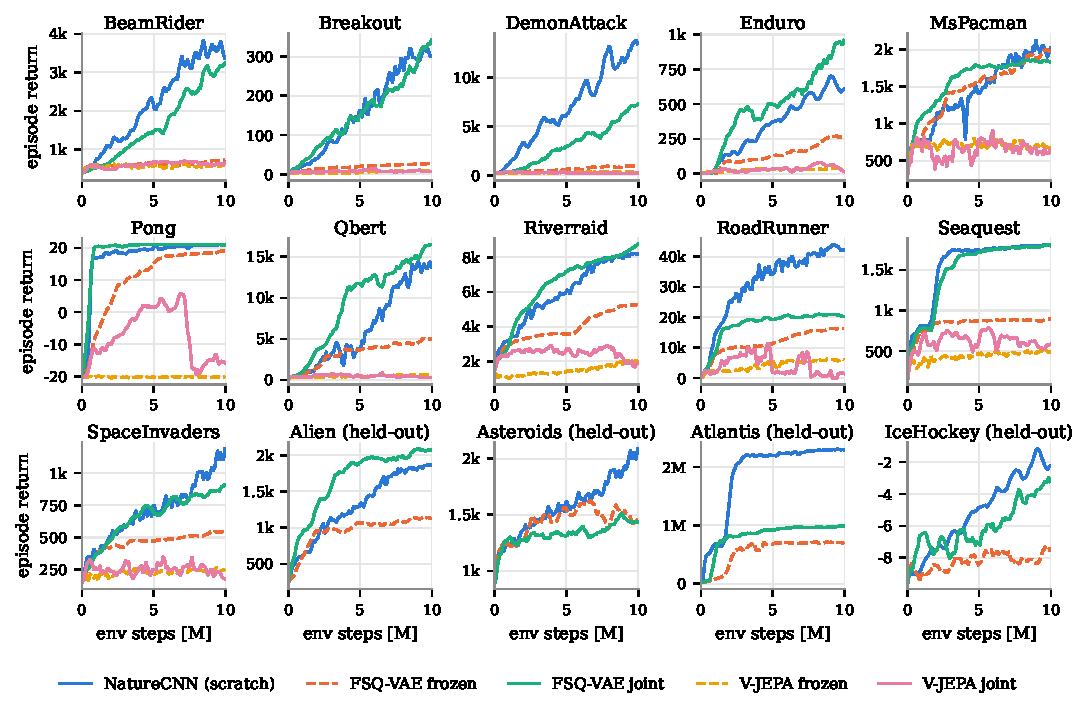
\includegraphics[width=0.9\textwidth]{figures/learning_curves.pdf}
\caption{Learning curves over 10\,M agent steps (100 bins; FSQ curves smoothed over five).
Solid: trained or fine-tuned encoders; dashed: frozen encoders.}
\label{fig:curves}
\end{figure}

\begin{table}[!htbp]
\centering
\caption{Sample efficiency: million steps until the learning curve first covers 50\% and 80\%
of the way from NatureCNN's initial to its final return (``--'': never). FSQ-J/F: FSQ-VAE
joint/frozen. Fastest in bold.}
\label{tab:sampleeff}
\footnotesize\setlength{\tabcolsep}{4pt}
\begin{tabular}{@{}lcccccc@{}}
\toprule
 & \multicolumn{3}{c}{50\% level} & \multicolumn{3}{c}{80\% level} \\
\cmidrule(lr){2-4}\cmidrule(lr){5-7}
Game & Nature & FSQ-J & FSQ-F & Nature & FSQ-J & FSQ-F \\
\midrule
\tabinput{tables/sample_eff_rows.tex}
\bottomrule
\end{tabular}
\end{table}

\paragraph{FSQ-VAE, Frozen.} With a frozen FSQ encoder, the agent still made progress in every
game, but considerably less (median HNS 0.31). It came close to the NatureCNN only on Pong and
MsPacman. Performance was weakest in games where the relevant object is small and fast
(DemonAttack, Breakout, BeamRider), where the agent reached only 6--11\% of the NatureCNN's
HNS, compared with 35--57\% on the remaining six games. I suspect that, even
with the motion-aware loss, reconstruction still spends most of its capacity on large areas.

\paragraph{Standard VAE and Residual VQ-VAE.} The Standard VAE scored lowest among the
autoencoders on every game, both frozen and fine-tuned (median HNS 0.06 and 0.36). The Residual
VQ-VAE scored below the FSQ-VAE on every game except MsPacman (fine-tuned), but fine-tuned it
still reached a higher median HNS than the NatureCNN (0.85 vs.\ 0.74). The gap to the FSQ-VAE
was largest on Breakout, DemonAttack and BeamRider, where the fine-tuned Residual VQ-VAE
reached only 28--52\% of the FSQ-VAE's return. These games have small, fast-moving objects,
which is consistent with its weaker reconstruction of moving pixels (\cref{sec:pretrain-res}).

\paragraph{V-JEPA.} Both V-JEPA agents learned very little (median HNS 0.05 frozen and 0.04
fine-tuned), even though the frozen critic predicted the returns reasonably well (explained
variance 0.56--0.97, where 1 means the critic predicts the returns perfectly and 0 means it is
no better than a constant). Fine-tuning was also unstable: on Pong, the agent reached $+8.4$ after
7\,M steps and then dropped back to $-15$. Suspecting that the 9\,216-dimensional feature was too large, I repeated all 22 seen-game runs
with the tokens averaged into a 256-dimensional feature. These runs also used separate encoders
for actor and critic, so the effects of the two changes cannot be separated. I then repeated the
frozen runs once more with a five times larger entropy bonus (\cref{tab:jepa-abl}). Neither the
pooled feature nor the larger bonus helped: the pooled frozen agent beat the
flattened one on only one game, the pooled fine-tuned policy became almost deterministic on ten
games, and the larger entropy bonus kept the policy random but prevented the critic from
learning.

\begin{table}[!htbp]
\centering
\caption{V-JEPA feature ablation (11 seen games): median HNS of the training return and of
the final policy on 30 test episodes, end-of-training critic explained variance and policy
entropy, and games on which the pooled variant beats the flattened one.}
\label{tab:jepa-abl}
\footnotesize\setlength{\tabcolsep}{3pt}
\begin{tabular}{@{}lcccccccc@{}}
\toprule
 & & & \multicolumn{2}{c}{median HNS} & expl. & & & \\
\cmidrule(lr){4-5}
Feature & mode & ent.\ coef. & train & test & var. & entropy & FPS & wins \\
\midrule
\tabinput{tables/jepa_ablation_rows.tex}
\bottomrule
\end{tabular}
\end{table}

\paragraph{Frozen vs.\ Fine-Tuned and Unseen Games.} For the FSQ encoder, fine-tuning
outperformed freezing on 13 of 15 games (all except MsPacman and Asteroids), in some cases by a
large factor (Breakout $12\times$, DemonAttack $7\times$). On the held-out games, it was better
on three of four (median HNS 0.45 vs.\ 0.21). However, the NatureCNN trained from scratch on
these games was ahead of it on Asteroids, Atlantis and IceHockey (median HNS 0.50), and the
pre-trained encoder was better only on Alien (2\,071 vs.\ 1\,850). All other pre-trained
encoders scored lower still (median HNS 0.01--0.21). Pre-training on eleven games therefore gave
no overall advantage on unseen games, although it did not prevent the agent from learning them.

\FloatBarrier
\subsection{World-Model Diagnostics}
\label{sec:jepa-diag}

A high similarity between predicted and actual latents can be misleading. A collapsed encoder
makes all latents similar, and since $s_{t+1}$ shares three frames with $s_t$, copying $z_t$
already achieves a high score. I therefore evaluated the V-JEPA on 64 sequences of five steps
and compared it against a copy baseline, an untrained model, and deliberately wrong actions
(\cref{tab:jepa}).

\begin{table}[!htbp]
\centering
\caption{V-JEPA diagnostics: seen games (validation split, true game embedding) and held-out
games (UNKNOWN embedding); chance or untrained values in brackets.}
\label{tab:jepa}
\footnotesize\setlength{\tabcolsep}{4pt}
\begin{tabular}{@{}lcc@{}}
\toprule
Diagnostic & 11 seen games & 4 held-out games \\
\midrule
Cos.\ sim.\ predictor / identity, $k=1$ & 0.987 / 0.974 & 0.939 / 0.971 \\
Cos.\ sim.\ predictor / identity, $k=5$ & 0.961 / 0.915 & 0.806 / 0.912 \\
Action sensitivity: sim.\ true $-$ wrong action & +0.0057 & +0.0001 \\
Attention on action / game token (uniform 0.026) & 0.029 / 0.046 & 0.026 / 0.055 \\
Inverse-dynamics accuracy & 55.9\% (12.9\%) & 1.8\% (5.6\%) \\
Effective rank / 256 & 52.5 (2.5) & 29.9 (1.5) \\
\bottomrule
\end{tabular}
\end{table}

On the seen games, the latent space did not collapse (effective rank 52.5 compared with 2.5 for
an untrained model), and the predictor outperformed copying at every step. The gap increased
from $+0.013$ after one step to $+0.046$ after five steps, when input and target no longer share any frames, so the model learned genuine dynamics. The action, however, had very little influence: giving the predictor a wrong action changed its output by
only 0.006, and the action token received barely more attention than an average token. The
game token received more attention (0.046, almost twice uniform), but the encoder could already
identify the game from the pixels: the latents form clusters by game (\cref{fig:tsne}). On the
held-out games, the predictor was worse than copying and the inverse head was below
chance, so the model learned the eleven training games rather than Atari in general.

\FloatBarrier
\subsection{Why the V-JEPA Failed with PPO}
\label{sec:jepa-fail}

Measured by its own training objectives, the V-JEPA performed well, yet PPO could not make use
of its features. \Cref{tab:jepa-fail} summarises the collected evidence, and \cref{fig:pca}
illustrates the central problem.

\begin{table}[!htbp]
\centering
\caption{Possible reasons why the V-JEPA encoder did not help PPO, with the evidence for each (from
\cref{sec:pretrain-res,sec:jepa-diag}, \cref{tab:jepa-abl} and \cref{fig:tsne}).}
\label{tab:jepa-fail}
\scriptsize\setlength{\tabcolsep}{3pt}
\newcolumntype{Y}[1]{>{\raggedright\arraybackslash}p{#1}}
\begin{tabular}{@{}Y{2.6cm}Y{5.0cm}Y{4.2cm}@{}}
\toprule
Possible reason & Evidence & Consequence for PPO \\
\midrule
Dynamics ignore the action & true vs.\ wrong action: $\Delta$cos.\ 0.006; action-token attention
  0.029 (uniform 0.026); \cref{fig:pca} & latent need not encode what the agent controls \\
Latents change slowly & $\cos(z_t,\bar z_{t+1})=0.974$; 0.915 five steps later;
  $14{\times}14$ patches & small, decisive sprite motion barely moves the feature \\
Organised by game & latents cluster by game (\cref{fig:tsne}); game token gets $1.8\times$
  uniform attention & capacity spent on
  information that is constant within a run \\
Specialised to pre-training games & held-out loss $3\times$ seen; held-out inverse accuracy
  below chance & tuned to expert states of eleven games \\
State, not action, information & critic expl.\ var.\ 0.56--0.97 while policy entropy stays
  high (1.53) & value readable, best action not \\
Little action variety in the data & expert's top action: 45\% (Qbert), 67\% (RoadRunner) of
  steps (\cref{tab:games}) & few examples of what \emph{other} actions would change \\
Not size or exploration & pooled 256-d feature, entropy bonus 0.05: no gain & rules out the
  simplest remedies \\
\bottomrule
\end{tabular}
\end{table}

\begin{figure}[!htbp]
\centering
\begin{subfigure}[t]{0.40\textwidth}\centering
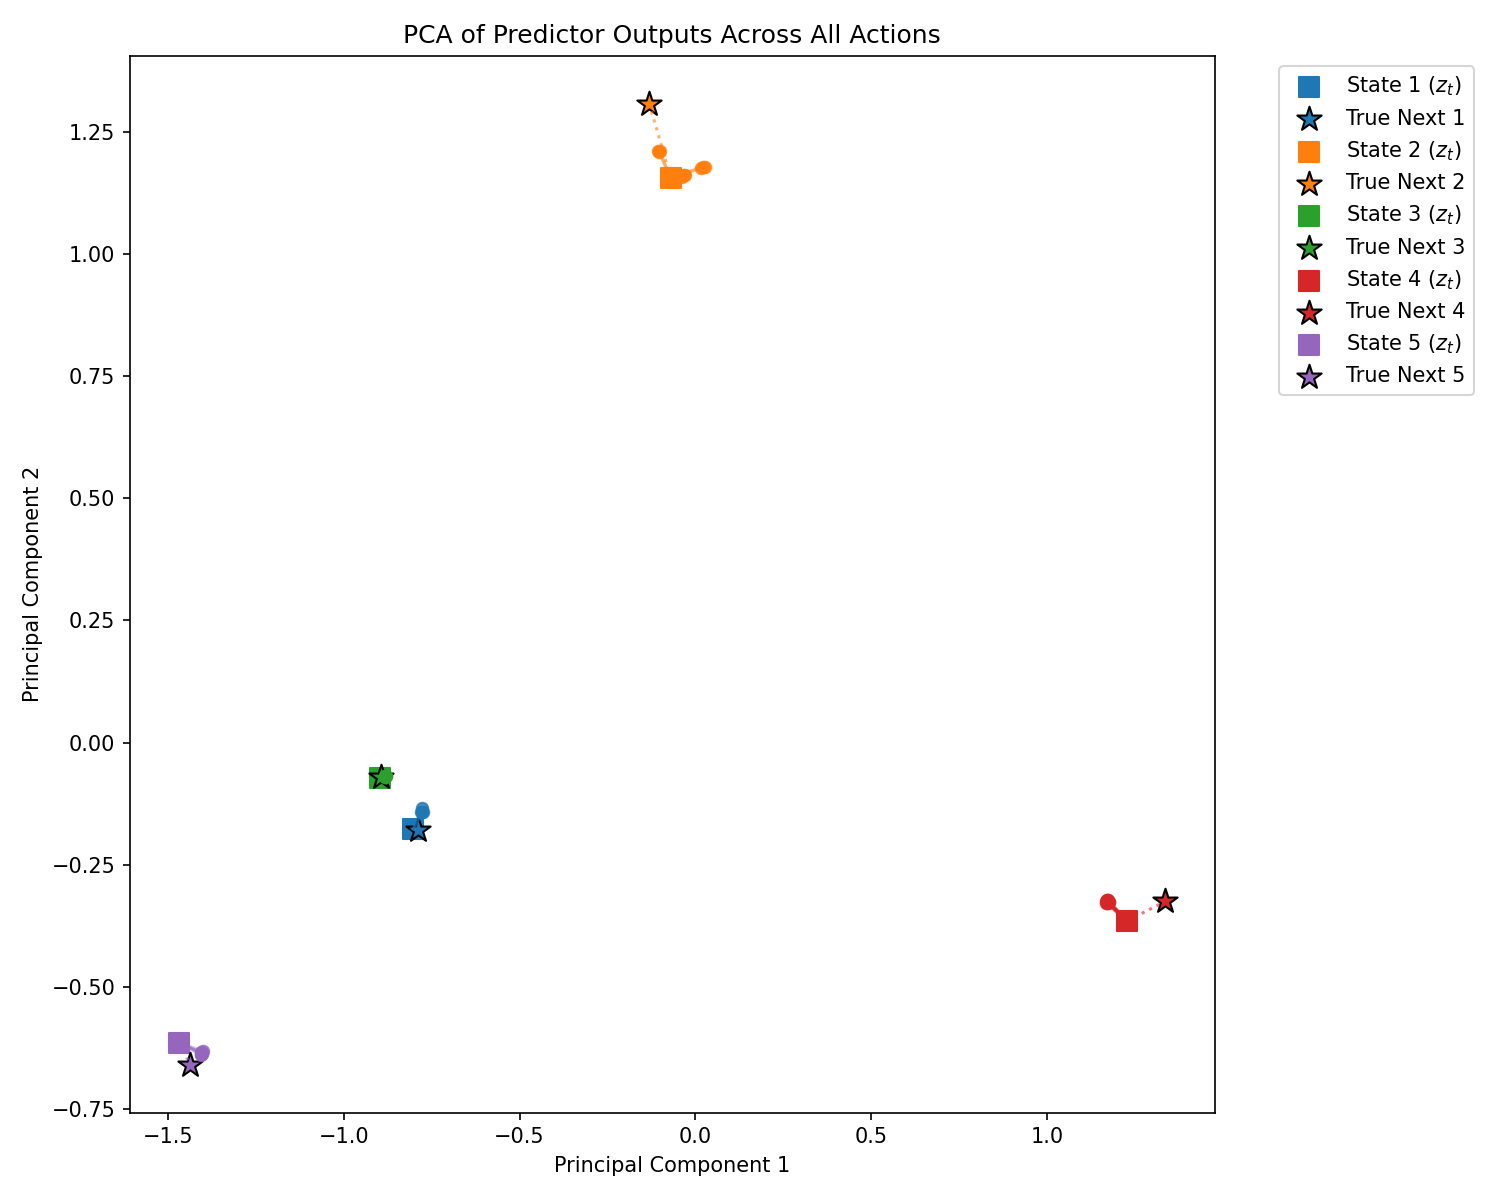
\includegraphics[width=\linewidth]{figures/pca_action_sensitivity.png}
\caption{PCA, predictions for all actions}\label{fig:pca}
\end{subfigure}\hfill
\begin{subfigure}[t]{0.40\textwidth}\centering
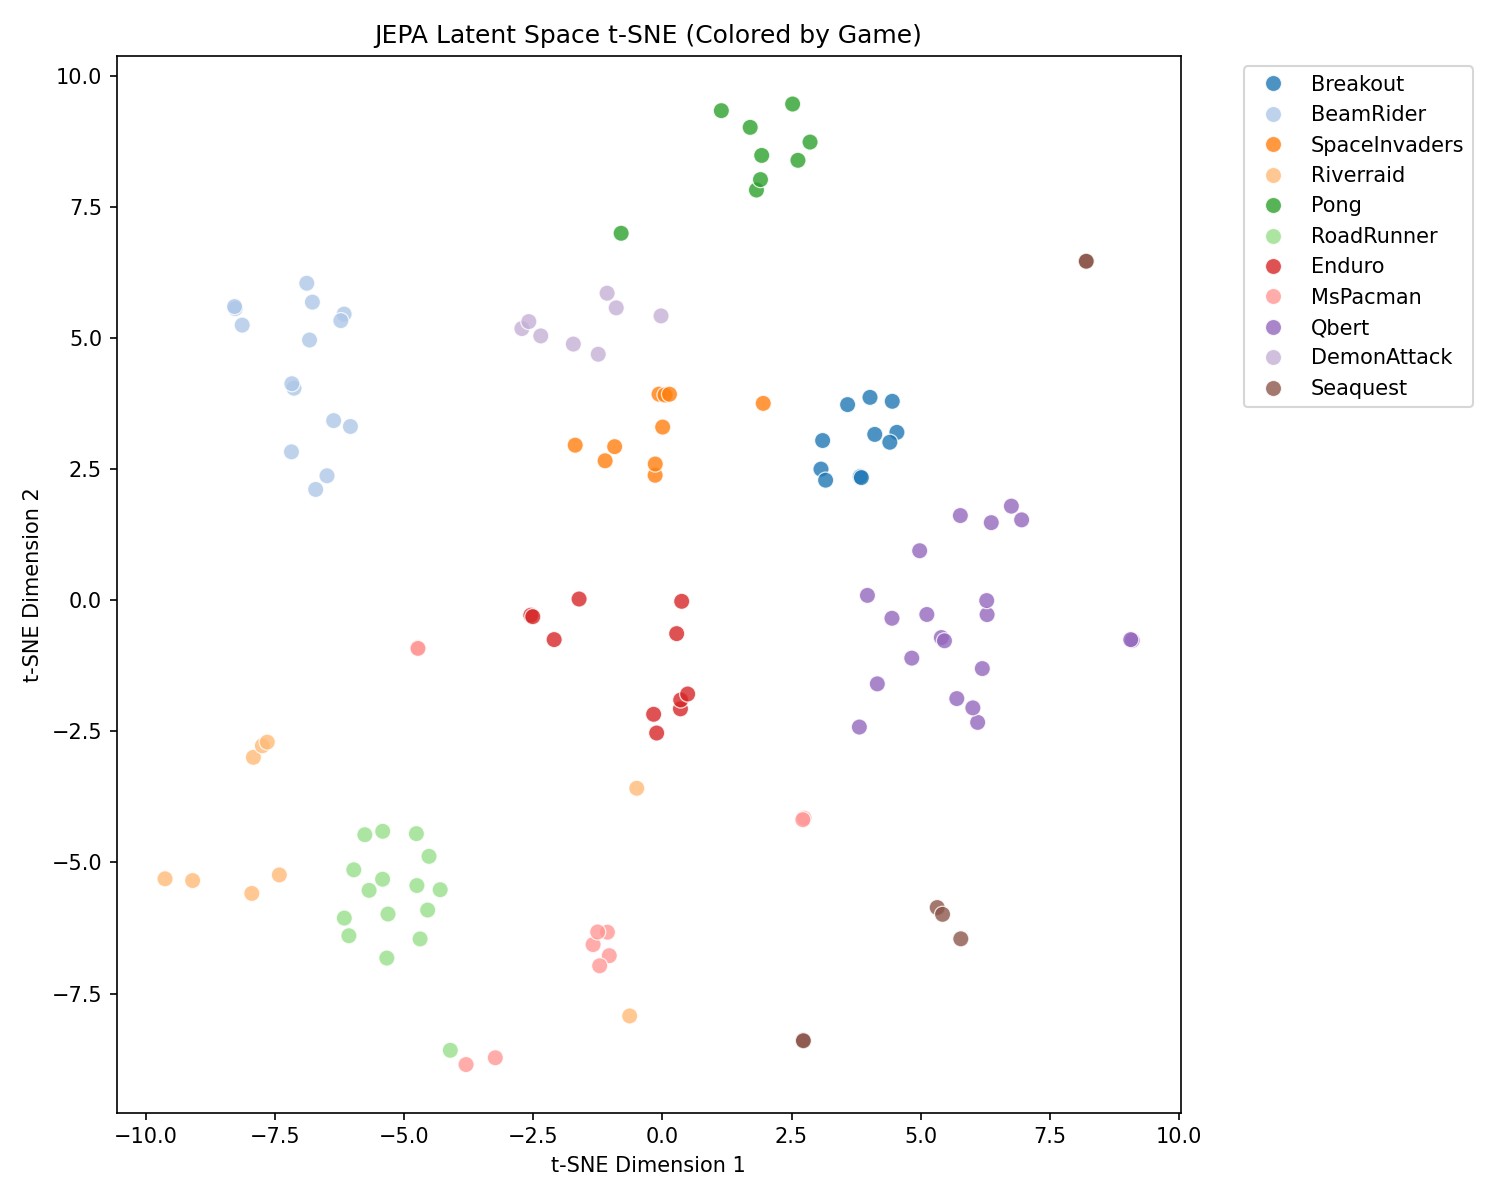
\includegraphics[width=\linewidth]{figures/jepa_tsne_by_game.png}
\caption{t-SNE, coloured by game}\label{fig:tsne}
\end{subfigure}
\caption{V-JEPA latents. (a)~PCA for five states: context $z_t$ (square), true next latent
(star) and the prediction for every valid action (dots). The predictions for all actions form
one tight cluster near $z_t$: the predictor hardly distinguishes between actions. (b)~t-SNE of
latents from the eleven seen games: they group by game.}
\label{fig:latents}
\end{figure}

My explanation is that the JEPA objective and PPO want different things. A JEPA only has to
predict what is \emph{predictable} about the next frame, so it can ignore small details that
have little effect on the latent error~\cite{lecun2022path,assran2023ijepa}. In Atari, however,
these details, like the exact position of the ball or a bullet, are what the agent needs to
act. A representation for control should capture what the agent's actions
change~\cite{gelada2019deepmdp}, and this is what my predictor modelled worst (\cref{fig:pca}).
The inverse loss was meant to help here, but it only trains the encoder (\cref{tab:grad}), and
the expert data contains few examples of other actions. The overlapping frames and the slowly
moving EMA target probably also push the model towards latents that change very little from one
step to the next. Such features seem to be enough for the critic to estimate how good a state
is (its explained variance was high), but probably too smooth for the policy to tell apart
states where the best action depends on a few pixels. Finally,
fine-tuning the 4.95\,M-parameter context encoder with PPO's learning rate was unstable, which
is consistent with reports that pre-trained visual features can be no better for control than
an encoder trained from scratch~\cite{hansen2022pretrained}.

\FloatBarrier
% =========================================================================
\section{Conclusion}
\label{sec:conclusion}

In this project, I investigated whether a single pre-trained encoder can serve as a universal
feature extractor for Atari games. I pre-trained VAE, VQ-VAE, FSQ-VAE and V-JEPA encoders on
expert data from eleven games and used them with PPO for 10\,M steps on these and four unseen
games, frozen or fine-tuned. The results give a partly positive answer.

The FSQ-VAE, pre-trained on eleven games without rewards, outperformed the Standard VAE on every
game and the Residual VQ-VAE on all but one, and proved to be a good initialisation
(\textbf{RQ1}). Fine-tuned with PPO, it achieved a higher median score than a NatureCNN trained
from scratch and learned faster on four games, although its final score was higher on only
four of eleven games and its mean score was lower. Frozen, it reached less than a third of that
median, so fine-tuning was clearly preferable (\textbf{RQ2}), probably because a frozen encoder
would need to keep every small detail that matters in every game, and nothing in a reward-free
objective forces it to. No pre-trained encoder gave an overall advantage on the unseen games: the
fine-tuned FSQ-VAE was better only on Alien, and the NatureCNN trained from scratch led on the
other three (\textbf{RQ3}). This is not surprising given only eleven pre-training games and
quite different held-out games (Asteroids is 95\% black). Freezing the V-JEPA encoder made PPO about a quarter
faster (854 vs.\ 677 steps per second), but it remained slower than the NatureCNN (976), so
freezing did not make the agent cheaper than training from scratch. The FSQ-VAE is easier to
interpret, because its decoder shows what the features contain (\textbf{RQ4}).

The V-JEPA learned a non-collapsed latent space and meaningful dynamics, but its objective
rewarded predicting what usually happens in a game rather than what the agent's actions change,
so its features were not useful for PPO, whether flattened or pooled. A practical lesson was that every bug in the V-JEPA pipeline still produced a plausible loss
curve, so checks such as the copy baseline and wrong actions were necessary.

The main limitations are the single seed and PPO hyper-parameters that were not re-tuned for
the pre-trained encoders. As a next step, I would repeat the main comparison with three seeds.
For the V-JEPA, smaller patches and a training signal in which the
action has a real effect (e.g.\ multi-step prediction or a reward head, as in TD-MPC2) appear
most promising, and the features should first be validated by predicting game-state variables
such as object positions. Using the FSQ grid inside a world
model~\cite{hafner2021dreamerv2,micheli2023iris} and pre-training on more games are further
directions. Whether a frozen encoder can work for all Atari games is still open after this
project.

\paragraph{Acknowledgements.}
I would like to thank Oleh Shkalikov for proposing and supervising this project, and the
Centre for Information Services and High Performance Computing (ZIH) at TU Dresden for the GPU
time on the \emph{Capella} cluster.

\bibliographystyle{splncs04-unsort}
\bibliography{references}

\end{document}
